%------------------------------------
% To be edited
%------------------------------------
\newcommand{\xfire}{X\textsubscript{FIRE} }
\newcommand{\documentname}{The \xfire Processor\\Architecture Specification}
\newcommand{\crev}{0.1}
\newcommand{\documentversion}{Rev. \crev}
\newcommand{\cryear}{2015}
\hyphenation{soft-ware hard-ware}
%------------------------------------

\documentclass[10pt,a4paper]{book}
\setlength{\parindent}{0pt}
\setlength{\parskip}{1ex plus 0.5ex minus 0.2ex}
\addtolength{\headsep}{0.5cm}
\usepackage[a4paper]{geometry} %,left=2.5cm,right=3.5cm
\usepackage{listings}
\lstloadlanguages{VHDL}
\usepackage[colorlinks=false]{hyperref}
\usepackage[english, activeacute]{babel}
\usepackage[utf8]{inputenc}
\usepackage{graphics}
\usepackage{graphicx}
\usepackage{subcaption}
\usepackage{rotating}
\usepackage{color}
\usepackage{longtable}
\usepackage{latexsym}
\usepackage{multicol}
\usepackage{multirow}
\usepackage{fancyhdr}
\usepackage{bytefield}
\usepackage{float}
\usepackage{tabu}
\usepackage{flafter}
\usepackage{morefloats}
\usepackage{fixltx2e}
\usepackage[verbose=false]{datatool}
\usepackage{datatool-base}
\usepackage{ifthen}
\usepackage{booktabs}

% Paquetes matematicos
\usepackage{amsfonts}
\usepackage{amsmath}
\usepackage{amssymb}
\usepackage{amsthm}
\usepackage{mathrsfs}

% Config para poder meter footnotes en las tablas:

\pagestyle{fancy}

%\usepackage{anysize}
%\marginsize{3cm}{4cm}{2.5cm}{3.5cm}

%---- Encabezado y pie de pagina general
\fancypagestyle{general}{
   \fancyhf{}
   \fancyfoot{}
   \fancyhead{}
   \fancyhead[LO]{\footnotesize{\leftmark}}
   \fancyhead[RE]{\footnotesize{\rightmark}}
   \fancyhead[RO]{\footnotesize{\thepage}}
   \fancyhead[LE]{\footnotesize{\thepage}}
   \renewcommand{\headrulewidth}{0pt}
   \renewcommand{\footrulewidth}{0pt}
}

\fancypagestyle{plain}{
   \fancyhf{}
   \fancyfoot{}
   \fancyhead{}
   \fancyfoot[RO]{\footnotesize{\thepage}}
   \fancyfoot[LE]{\footnotesize{\thepage}}
   \renewcommand{\headrulewidth}{0pt}
   \renewcommand{\footrulewidth}{0pt}
}

%---- Encabezado y pie de pagina de la caratula
\fancypagestyle{carat} {
   \fancyhf{}
   \fancyfoot{}
   \fancyhead{}
   \fancyhead[LO]{\scalebox{0.15}{
\includegraphics[angle=0]{./figures/logo_lab_ue_3.png}}}
   \fancyhead[RE]{}
   \fancyhead[RO]{\scalebox{0.5}{
\includegraphics[angle=0]{./figures/logo_fiuba.jpg}}}
   \fancyhead[LE]{}
   \fancyhead[CE]{}
   \fancyfoot[CO]{\textcircled{c} Lab-$\mu$E, FIUBA. \cryear.}
   \renewcommand{\headrulewidth}{0pt}
   \renewcommand{\footrulewidth}{1pt}
}

%---- Quito los encabezados y pies de pagina en las hojas vacias
\makeatletter
  \def\cleardoublepage{\clearpage\if@twoside \ifodd\c@page\else
  \vspace*{\fill}
    \thispagestyle{empty}
    \newpage
    \if@twocolumn\hbox{}\newpage\fi\fi\fi}
\makeatother

%---- Espaciado en el indice entre el numero y el titulo
\makeatletter
\renewcommand*{\l@subsection}{\@dottedtocline{1}{3.8em}{3.5em}}
\renewcommand*{\l@figure}{\@dottedtocline{1}{1.5em}{3.3em}}
\renewcommand*{\l@table}{\@dottedtocline{1}{1.5em}{2.8em}}
\makeatother

%---- Formateo del codigo VHDL
\lstset{
   %extendedchars=true,%
   %labelstep=0,
   %labelsep=3ex,
   %frame=trbl,
   %frameround=tttt,
   %framespread=-3ex,
   %framerulecolor=colorFondoListado,
   %backgroundcolor=colorFondoListado,
   captionpos=b,
   breaklines=true,
   %linewidth=0.98\linewidth,
   %indent=5ex,
   tabsize=4,
   %labelstyle=\small\ttfamily,
   basicstyle=\scriptsize\sffamily,
   %numberstyle=\small\sffamily,
   identifierstyle=\scriptsize\sffamily,
   commentstyle=\scriptsize\itshape,
   stringstyle=\scriptsize\sffamily,
   keywordstyle=\scriptsize\bfseries\sffamily,
   ndkeywordstyle=\scriptsize\bfseries\sffamily,
   showstringspaces=false,
   flexiblecolumns=false
   visiblespaces=false
   %stringspaces=false
}

%---- Encabezado y pie de pagina por defecto
\pagestyle{general}

%---- Matematica
% \newtheorem{defi}{Definici\'on}
% \newtheorem{teor}{Teorema}
% \newtheorem{prop}{Proposici\'on}
% \newtheorem{lema}{Lema}
% \newtheorem{cor}{Corolario}
% \DeclareMathOperator{\sen}{sen}
% \DeclareMathOperator{\supr}{sup}
% \DeclareMathOperator{\sgn}{sgn}
% \DeclareMathOperator{\lip}{lip}
% \DeclareMathOperator{\codim}{codim}
% \DeclareMathOperator{\gen}{gen}
% \DeclareMathOperator{\im}{Im}
% \DeclareMathOperator{\nuc}{Nu}
% \DeclareMathOperator{\ind}{ind}
% \DeclareMathOperator{\dom}{Dom}
% \DeclareMathOperator{\real}{Real}
% \DeclareMathOperator{\imag}{Imag}

%---- Para no separar en SILABAS se activa el comando siguiente
\hyphenpenalty=10000

\begin{document}

% \renewcommand{\contentsname}{\'Indice}
% \renewcommand{\partname}{Parte}
% \renewcommand{\chaptername}{Cap\'itulo}
% \renewcommand{\appendixname}{Ap\'endice}
% \renewcommand{\bibname}{Referencias}
% \renewcommand{\figurename}{Figura}
% \renewcommand{\listfigurename}{\'Indice de Figuras}
% \renewcommand{\tablename}{Tabla}
% \renewcommand{\listtablename}{\'Indice de Tablas}

\enlargethispage{2cm}
\thispagestyle{carat}

\

\rule{14.8cm}{3pt}

\

\

\begin{flushright}{\Huge{\textbf{\documentname}}}\end{flushright}

\

\

\ \normalsize

\

\

\begin{flushright}

\includegraphics[scale=0.5]{./figures/xfire.png}
\end{flushright}

\

\

\

\

\

\begin{flushright}
\documentversion\\
\today\\
\end{flushright}

\

\

\

\

\

\

\

\newpage
\thispagestyle{empty}

\

\newpage
\section*{Abstract}
\label{sec:abstract}

\


This document contains all the functional specifications needed for designing, implementing
and verifying the \xfire Processor Architecture.
\newpage
\thispagestyle{empty}

\

\newpage
\section*{Revision history}
\label{sec:rev}

\

\begin{center}
\begin{tabular}{|c|c|c|c|}
\hline
\textbf{Rev.} & \textbf{Date} & \textbf{Author/s} & \textbf{Description}\\
\hline
\hline
1.0 & August 31, 2015 & Alpago, Octavio      & First draft version. \\
    &                 & Natale, Luciano      &  \\
    &                 & Luciano Natale       & \\
    &                 & Zacchigna, Federico Giordano & \\
\hline
\end{tabular}
\end{center}

\newpage
\thispagestyle{empty}

\

\tableofcontents
\listoffigures
\listoftables
\section{About This Document}
\label{sec:about}

\subsection{Introduction}
\label{ssec:introduction}
Welcome to the \xfire Processor Architecture! The \xfire (pronoiced ``Crossfire'') Processor Architechture is targeted
to be synthesized on FPGA and ASICs and its objective is to provide a solution for embedded systems. The processor is designed under the full RISC
philosophy and is mainly focused on providing a simple and implementation agnositc architecture.

This manual describes the architechture, the instruction set, the internal registers, the addressing modes, the supported data types, the memory model,
the peripheral interface, exceptions and interruptions. This manual does not describe neither implementation nor details such as pipeline,
cache and other optimizations, leaving those details to the implementation itself.

\subsection{List of contributors}
\label{ssec:contributors}
By alphabetic order:
\begin{itemize}
\item Alpago, Octavio - oalpago@gmail.com
\item Natale, Luciano - luchonat@gmail.com
\item Sanca, Gabriel - gandres.sanca@gmail.com
\item Zacchigna, Federico Giordano  - federico.zacchigna@gmail.com
\end{itemize}

\subsection{Conventions}
\label{ssec:conventions}


\chapter{Architecture description}
\section{Data types}
\label{sec:data_types}

Integer supported data types are: \emph{byte} (8 bits), \emph{half} (16 bits), \emph{word} (32 bits), \emph{double word} (64 bits).
Floating point supported data types are: \emph{single-precision} (32 bits) and \emph{double-precision} (64 bits). Data sizes are shown in
figure \ref{fig:data_sizes}.

\begin{itemize}
   \item \emph{Byte} is also referred as \emph{char}.
   \item \emph{Half} is also referred as \emph{short}.
   \item \emph{Word} is also referred as \emph{integer}.
   \item \emph{Double word} is also referred as \emph{long}.
   \item \emph{Single-precision floating point} is also referred as \emph{float}.
   \item \emph{Double-precision floating point} is also referred as \emph{double}.
\end{itemize}

\begin{figure}
  \begin{center}
    \begin{bytefield}[bitwidth=0.6em,endianness=big]{74}
      \bitheader{0,7,15,31,63}\\
      \bitbox[]{10}{Byte, char}   & \bitbox[]{56}{} & \bitbox[lrbt]{8}{}\\
      \bitbox[]{10}{Half, short}  & \bitbox[]{48}{} & \bitbox[lrbt]{16}{}\\
      \bitbox[]{10}{Word}         & \bitbox[]{32}{} & \bitbox[lrbt]{32}{}\\
      \bitbox[]{10}{Long}         & \bitbox[lrbt]{64}{}\\
      \bitbox[]{10}{Float}        & \bitbox[]{32}{} & \bitbox[lrbt]{32}{}\\
      \bitbox[]{10}{Double}       & \bitbox[lrbt]{64}{}\\
    \end{bytefield}
    \caption{Data sizes.}
    \label{fig:data_sizes}
  \end{center} 
\end{figure}


\section{Internal Registers}
\label{sec:registers}
The reset state of all the registers is 0 including the special purpose registers. Exception to this rule is the L0
register when implemented, whose reset value is 0x800000000.

\subsection{General Purpose Registers}
\label{ssec:gprs}
\begin{itemize}
   \item There are 32 general purpose registers (GPRs) named R0, R1, $\ldots$ R31.
   \item The GPRs can be used as even-odd pairs holding long integer registers named R0, R2, R4, $\ldots$, R30.
   \item Each GPR has 4 flag bits: carry (C), negative (N), overflow (V), zero (Z) which store the ALU operation status. The negative
         flag is implicit and corresponds to the MSB of the GPR (bit 31).
%    \item When loading data into a GPR from memory, negative (N) and zero (Z) flags are consistent with the data loaded, and carry (C)
%          and overflow (V) are zeroed.
%    \item When an ALU operation writes back double words on pair registers, the even register holding the lower bits of the long data has its carry (C) and
%          overflow (V) flags zeroed; and negative (N) and zero (Z) flags consistent with the data hold by the register, the odd register holding the upper bits of the
%          long data, has all flags consistent with the operation.
   \item When loading data into a GPR from memory, carry (C), overflow(V) and zero (Z) flags are left unmodified; negative (N) flag is implicit in the data
	 loaded in the register.
   \item When an ALU operation writes back double words on pair of registers, the even register holding the lower bits of the long data has its carry (C),
         overflow (V) and zero (Z) flags unmodified; negative (N) flag is implicit in the data hold by the register, the odd register holding the upper bits
         of the long data, has all flags consistent with the operation.
   \item Byte and half data types are loaded into the low portion of GPRs from memory with either zeros or sign bit replicated to fill
         the 32 bits depending on the instruction.
   \item There are 32 single-precision floating point registers (FPRs) named F0, F1, $\ldots$, F31.
   \item The FPRs can be used as even-odd pairs holding double-precision floating point registers named F0, F2, F4, $\ldots$, F30.
   \item Each FPR has 4 flag bits: is-a-number (A), is-infinity (I), negative (N), zero (Z) which store the FPU operation status. The negative
         flag is implicit and corresponds to the MSB of the FPR (bit 31).
%    \item When loading data into a FPR from memory, all flags are consistent with the data loaded.
%    \item When an FPU operation writes back double floats on pair registers, the even register holding the lower bits of the double float has all its flags consistent
%          with the floating point number represented by this register, the odd register holding the upper bits of the double float has all its flags consistent with
%          the operation.
   \item When loading data into a FPR from memory, is-a-number (A), is-infinity (I), and zero (Z) are left unmodified; negative (N) flag is implicit in
         the data loaded in the register.
   \item When an FPU operation writes back double floats on pair registers, the even register holding the lower bits of the double float has its is-a-number
         (A), is-infinity (I), and zero (Z) flags unmodified; negative (N) flag is implicit in the data loaded in the register, the odd register holding the
         upper bits of the double float has all its flags consistent with the operation.
\end{itemize}

\subsection{Special Purpose Registers}
\label{ssec:sprs}
The procesor provides a set of special registers, some of them are accesible with special instructions. Special registers are:
\begin{itemize}
   \item The config register (CFG) is 6 bits wide and stores the configuration status of the processor. Its content is set and read with
         special register instructions. Since special moving instructions transfer 32 bits, bits from 31 down to 6 are discarded on write,
         and return zero on read.

         Bit 0 stores the execution mode. If unset, the processor is running in supervisor mode. If set, it is running in user mode.
         Read section \ref{sec:modes} for more information on execution modes.

         Bit 1 stores the configuration support for nested exceptions. If unset, the processor does not provide support for nested exceptions,
         while if set, it does.
         Read subsection \ref{ssec:exception_handling} for more information on the nested exceptions support.

         Bits 3 down to 2 selects the system tick timer operation mode. Bit 2 selects free running mode. If unset, the system tick timer is in free runing mode. If set
         is in auto stop mode. When running in auto stop mode, bit 3 works as system tick timer start. This bit is not sticky, meaning that it goes back to '0' one
         clock cycle after it was written and always returns '0' on read.
         Read subsection \ref{ssec:sys_tick} for more information on the systick exception.

         Bits 5 down to 4 selects the rounding mode for floating point operations. The encoding is as follows:
         \begin{itemize}
          \item '00’: RN - Round to nearest
          \item '01’: RZ - Round towards zero
          \item '10’: RP - Round towards plus infinity
          \item '11’: RM - Round towards minus infinity
         \end{itemize}
   \item The system timer period register (STP) is a 22 bits register that configures the system timer reload value.
         Read subsection \ref{ssec:sys_tick} for more information on the systick exception.
   \item The mask register (MR) is 33 bits wide and provides the mechanisms to enable or disable the corresponding source of interruption
         or cause. The most significant bit is the global mask bit. This bit is not software accesible; this means that instructions
         cannot read or write to this special bit and its content is set and read automatically by the architecture. When it is set, all
         exceptions are disabled. Its content is set and read with special register instructions. Read section \ref{sec:exceptions}
         for more information on this register.
   \item The instruction register (IR) is 32 bits wide and stores the opcode of the instruction that is being executed. Its content is
         read with special register instructions. A writing operation on this register has no effect.
   \item The system timer register (TMR) is 32 bits wide and corresponds to a 32 bits down counter that generates the systick exception
         when reaches zero. The reload value of the system timer can be configured trough the STP register. This register is read only for software:
         a writing operation has no efect on this register. Read subsection \ref{ssec:sys_tick} for more information on this register.
   \item The peripheral write data register (PWD) is 32 bits wide and provides outgoing communication with peripherals. Its content is
         set and read with special register instructions.
   \item The peripheral write address register (PWA) is 32 bits wide and provides addressing for peripherals. Its content is
         set and read with special register instructions.
   \item The peripheral read data register (PRD) is 32 bits wide and provides incoming communication with peripherals. Its content is
         read with special register instructions. A writing operation on this register has no effect.
   \item The peripheral read address register (PRA) is 32 bits wide and provides incomming identification of peripherals. Its content is read
         with special register instructions. A writing operation on this register has no effect.
   \item The program counter (PC) is 30 bits wide addressing a memory space which ranges from \texttt{0x00000000} to \texttt{0xFFFFFFFC}.
         This register is not software addressable. The current address is given by $4*PC$.
   \item The cause register (CR) is 32 bits wide and stores the cause of exceptions and interrupts. Each bit represents a different
         exception cause / interrupt source. When an exception or interrupt condition is detected, the corresponding bit must be set, and
         shall remain set until the event is handled. The hardware is responsible of reseting the corresponding bit when execution of the
         handler is started. This register is not software addressable. Read section \ref{sec:exceptions} for more information on this register.
   \item The link register stack (LRS) is a set of 32 registers named $L0,L1,\ldots,L31$ which store the return address (PC + 1) value \textbf{only}
         from exceptions. Each register is 36 bits wide. This register file is optional and adds support for nested exceptions. If not supported,
         then one link register (L0) must be implemented. These registers are not software addressable. Read subsection \ref{ssec:exception_handling} for
         more information.
   \item The exception stack pointer (ESP) is a 5 bits wide register and points to the top of the LRS. This register is optional and adds support for
         nested interruptions. Read subsection \ref{ssec:exception_handling} for more information.
\end{itemize}

The structure and organization of registers is shown in Tables \ref{tbl:general_reg_organization} and \ref{tbl:special_reg_organization}.

\begin{figure}
  \begin{center}
    \begin{bytefield}[bitwidth=0.9em,endianness=big]{40}
      \bitheader{0-34}\\
      \bitbox[]{4}{R0}        & \bitbox[r]{1}{}    & \bitbox{1}{C}      & \bitbox{1}{V}      & \bitbox{1}{Z}      & \bitbox{1}{N} & \bitbox[rbt]{31}{}\\
      \bitbox[]{4}{R1}        & \bitbox[r]{1}{}    & \bitbox{1}{C}      & \bitbox{1}{V}      & \bitbox{1}{Z}      & \bitbox{1}{N} & \bitbox[rbt]{31}{}\\
      \bitbox[]{4}{}          & \bitbox[r]{1}{}    & \bitbox[lrt]{1}{}  & \bitbox[lrt]{1}{}  & \bitbox[lrt]{1}{}  & \bitbox[ltr]{1}{} & \bitbox[rt]{31}{} \\
      \bitbox[]{4}{$\vdots$}  & \bitbox[r]{1}{}    & \bitbox[lr]{1}{$\vdots$}        & \bitbox[lr]{1}{$\vdots$} & \bitbox[lr]{1}{$\vdots$} & \bitbox[lr]{1}{$\vdots$} & \bitbox[r]{31}{$\vdots$} \\
      \bitbox[]{4}{}          & \bitbox[r]{1}{}    & \bitbox[lrb]{1}{}  & \bitbox[lrb]{1}{}  & \bitbox[lrb]{1}{}  & \bitbox[lbr]{1}{} & \bitbox[rb]{31}{} \\
      \bitbox[]{4}{R31}       & \bitbox[r]{1}{}    & \bitbox{1}{C}      & \bitbox{1}{V}      & \bitbox{1}{Z}      & \bitbox{1}{N} & \bitbox[rbt]{31}{}\\
      \bitbox[]{40}{} \\

      \bitheader{0-34}\\
      \bitbox[]{4}{F0}        & \bitbox[r]{1}{}      & \bitbox{1}{A}      & \bitbox{1}{I}      & \bitbox{1}{Z}      & \bitbox{1}{N} & \bitbox[rbt]{31}{}\\
      \bitbox[]{4}{F1}        & \bitbox[r]{1}{}      & \bitbox{1}{A}      & \bitbox{1}{I}      & \bitbox{1}{Z}      & \bitbox{1}{N} & \bitbox[rbt]{31}{}\\
      \bitbox[]{4}{}          & \bitbox[r]{1}{}      & \bitbox[lrt]{1}{} & \bitbox[lrt]{1}{}  & \bitbox[lrt]{1}{}  & \bitbox[ltr]{1}{} & \bitbox[rt]{31}{} \\
      \bitbox[]{4}{$\vdots$}  & \bitbox[r]{1}{}      & \bitbox[lr]{1}{$\vdots$}   & \bitbox[lr]{1}{$\vdots$} & \bitbox[lr]{1}{$\vdots$} & \bitbox[lr]{1}{$\vdots$} & \bitbox[r]{31}{$\vdots$} \\
      \bitbox[]{4}{}          & \bitbox[r]{1}{}      & \bitbox[lrb]{1}{} & \bitbox[lrb]{1}{}  & \bitbox[lrb]{1}{}  & \bitbox[lbr]{1}{} & \bitbox[rb]{31}{} \\
      \bitbox[]{4}{F31}       & \bitbox[r]{1}{}      & \bitbox{1}{A}      & \bitbox{1}{I} & \bitbox{1}{Z} & \bitbox{1}{N} & \bitbox[rbt]{31}{}\\
      \bitbox[]{40}{} \\

    \end{bytefield}
  \end{center}
  \caption{General registers structure and organization.}
  \label{fig:general_reg_organization}
\end{figure}

\begin{figure}
  \begin{center}
    \begin{bytefield}[bitwidth=0.9em,endianness=big]{40}

      \bitheader{0-5}\\
      \bitbox[]{4}{CFG}     & \bitbox[]{30}{}     & \bitbox[lrtb]{2}{} & \bitbox[lrtb]{2}{} & \bitbox[lrtb]{1}{}  & \bitbox[lrtb]{1}{}\\
      \bitbox[]{40}{} \\

      \bitheader{0-21}\\
      \bitbox[]{4}{STP}      & \bitbox[]{14}{}      & \bitbox{22}{}\\
      \bitbox[]{40}{} \\

      \bitheader{0-32}\\
      \bitbox[]{4}{MR}     & \bitbox[]{3}{}
                           & \bitbox[lrtb]{1}{} & \bitbox[lrtb]{1}{} & \bitbox[lrtb]{1}{} & \bitbox[lrtb]{1}{} & \bitbox[lrtb]{1}{}
                           & \bitbox[lrtb]{1}{} & \bitbox[lrtb]{1}{} & \bitbox[lrtb]{1}{} & \bitbox[lrtb]{1}{} & \bitbox[lrtb]{1}{}
                           & \bitbox[lrtb]{1}{} & \bitbox[lrtb]{1}{} & \bitbox[lrtb]{1}{} & \bitbox[lrtb]{1}{} & \bitbox[lrtb]{1}{}
                           & \bitbox[lrtb]{1}{} & \bitbox[lrtb]{1}{} & \bitbox[lrtb]{1}{} & \bitbox[lrtb]{1}{} & \bitbox[lrtb]{1}{}
                           & \bitbox[lrtb]{1}{} & \bitbox[lrtb]{1}{} & \bitbox[lrtb]{1}{} & \bitbox[lrtb]{1}{} & \bitbox[lrtb]{1}{}
                           & \bitbox[lrtb]{1}{} & \bitbox[lrtb]{1}{} & \bitbox[lrtb]{1}{} & \bitbox[lrtb]{1}{} & \bitbox[lrtb]{1}{}
                           & \bitbox[lrtb]{1}{} & \bitbox[lrtb]{1}{} & \bitbox[lrtb]{1}{}\\
      \bitbox[]{40}{} \\

      \bitheader{0-31}\\
      \bitbox[]{4}{IR}      & \bitbox[]{4}{}      & \bitbox{32}{}\\
      \bitbox[]{40}{} \\

      \bitheader{0-31}\\
      \bitbox[]{4}{TMR}     & \bitbox[]{4}{}      & \bitbox{32}{}\\
      \bitbox[]{40}{} \\

      \bitheader{0-31}\\
      \bitbox[]{4}{PWD}      & \bitbox[]{4}{}      & \bitbox{32}{}\\
      \bitbox[]{40}{} \\

      \bitheader{0-31}\\
      \bitbox[]{4}{PWA}      & \bitbox[]{4}{}      & \bitbox{32}{}\\
      \bitbox[]{40}{} \\

      \bitheader{0-31}\\
      \bitbox[]{4}{PRD}      & \bitbox[]{4}{}      & \bitbox{32}{}\\
      \bitbox[]{40}{} \\

      \bitheader{0-31}\\
      \bitbox[]{4}{PRA}      & \bitbox[]{4}{}     & \bitbox{32}{}\\
      \bitbox[]{40}{} \\

      \bitheader{0-29}\\
      \bitbox[]{4}{PC}      & \bitbox[]{6}{}      & \bitbox{30}{}\\
      \bitbox[]{40}{} \\

      \bitheader{0-31}\\
      \bitbox[]{4}{CR}     & \bitbox[]{4}{}
                           & \bitbox[lrtb]{1}{} & \bitbox[lrtb]{1}{} & \bitbox[lrtb]{1}{} & \bitbox[lrtb]{1}{} & \bitbox[lrtb]{1}{}
                           & \bitbox[lrtb]{1}{} & \bitbox[lrtb]{1}{} & \bitbox[lrtb]{1}{} & \bitbox[lrtb]{1}{} & \bitbox[lrtb]{1}{}
                           & \bitbox[lrtb]{1}{} & \bitbox[lrtb]{1}{} & \bitbox[lrtb]{1}{} & \bitbox[lrtb]{1}{} & \bitbox[lrtb]{1}{}
                           & \bitbox[lrtb]{1}{} & \bitbox[lrtb]{1}{} & \bitbox[lrtb]{1}{} & \bitbox[lrtb]{1}{} & \bitbox[lrtb]{1}{}
                           & \bitbox[lrtb]{1}{} & \bitbox[lrtb]{1}{} & \bitbox[lrtb]{1}{} & \bitbox[lrtb]{1}{} & \bitbox[lrtb]{1}{}
                           & \bitbox[lrtb]{1}{} & \bitbox[lrtb]{1}{} & \bitbox[lrtb]{1}{} & \bitbox[lrtb]{1}{} & \bitbox[lrtb]{1}{}
                           & \bitbox[lrtb]{1}{} & \bitbox[lrtb]{1}{}\\
      \bitbox[]{40}{} \\

      \bitheader{0-35}\\
      \bitbox[]{4}{L0}       & \bitbox{6}{}             & \bitbox{30}{}\\
      \bitbox[]{4}{L1}       & \bitbox{6}{}             & \bitbox{30}{}\\
      \bitbox[]{4}{}         & \bitbox[lrt]{6}{}        & \bitbox[lrt]{30}{}\\
      \bitbox[]{4}{$\vdots$} & \bitbox[lr]{6}{$\vdots$} & \bitbox[lr]{30}{$\vdots$}\\
      \bitbox[]{4}{}         & \bitbox[lrb]{6}{}        & \bitbox[lrb]{30}{}\\
      \bitbox[]{4}{L31}      & \bitbox{6}{}             & \bitbox{30}{}\\
      \bitbox[]{40}{} \\

      \bitheader{0-4}\\
      \bitbox[]{4}{ESP}     & \bitbox[]{31}{}      & \bitbox{5}{}\\
      \bitbox[]{40}{} \\

    \end{bytefield}
    \caption{Special registers structure and organization.}
    \label{tbl:special_reg_organization}
  \end{center}
\end{figure}


\subsubsection{Addressing of Special Registers}
\label{sssec:sprs_addressing}
Software addressable special registers are set and read with special register instructions called \emph{movi2s} and \emph{movs2i}. For
more informtion on this instructions, read section \ref{sec:isa}.
Special registers addressing is shown in Table \ref{tbl:special_reg_addresses}.

\begin{table}
  \begin{center}
    \begin{tabu} to \textwidth {|X|X[c]|X[c]|X[c]|X|X|}
    \hline
    \rowfont[c]\bfseries
    Register Name & Mapped Address & Hardware Size [bits] & Software Size [bits] & Hardware Access & Software Access \\
    \hline
    \hline
    CFG      & 0x00     & 6        & 32       & Read only      & Read-Write     \\
    \hline
    STP      & 0x01     & 22       & 32       & Read only      & Read-Write     \footnote{10 higher bits return zero on read and are zeroed on write.} \\
    \hline
    MR       & 0x02     & 33       & 32       & Read-Write     & Read-Write     \footnote{Except bit 33 which is non software accessible.}\\
    \hline
    IR       & 0x03     & 32       & 32       & Read-Write     & Read only      \\
    \hline
    TMR      & 0x04     & 32       & 32       & Read-Write     & Read only      \\
    \hline
    PWD      & 0x05     & 32       & 32       & Non accessible & Read-Write     \\
    \hline
    PWA      & 0x06     & 32       & 32       & Non accessible & Read-Write     \\
    \hline
    PRD      & 0x07     & 32       & 32       & Read only      & Read only      \\
    \hline
    PRA      & 0x08     & 32       & 32       & Read only      & Read only      \\
    \hline
    PC       & NA       & 30       & 0        & Read-Write     & Non accessible \\
    \hline
    CR       & NA       & 32       & 0        & Read-Write     & Non accessible \\
    \hline
    L0       & NA       & 36       & 0        & Read-Write     & Non accessible \\
    \hline
    $\vdots$ & $\vdots$ & $\vdots$ & $\vdots$ & $\vdots$       & $\vdots$       \\
    \hline
    L31      & NA       & 36       & 0        & Read-Write     & Non accessible \\
    \hline
    ESP      & NA       & 5        & 0        & Read-Write     & Non accessible \\
    \hline
    \end{tabu}
  \caption{Special registers addressing.}
  \label{tbl:special_reg_addresses}
  \end{center}
\end{table}

\section{Ports Interface}
\label{sec:ports}
\begin{table}
\begin{center}
\begin{tabu} to \textwidth {|X[l]|X[2.5,l]|X[c]|X[c]|}
\hline
\rowfont[c]\bfseries
Port name & Description & Size (Bits) & Type\\
\hline
\hline
arst         & Asynchronous high level active reset         & 1  & Input   \\
\hline
clk          & Posedge active clock                         & 1  & Input   \\
\hline
ena          & High level active synchronous enable         & 1  & Input   \\
\hline
dm\_wr\_data & Data memory write data bus                   & 32 & Output  \\
\hline
dm\_rd\_data & Data memory read data bus                    & 32 & Input   \\
\hline
dm\_address  & Data memory address bus                      & 32 & Output  \\
\hline
dm\_wr\_ena  & High level active data memory write enable   & 1  & Output  \\
\hline
im\_rd\_data & Instruction memory read data bus             & 32 & Input   \\
\hline
im\_address  & Instruction memory address bus               & 32 & Output  \\
\hline
us           & User/Supervisor execution mode ('1': user, '0': supervisor)  & 1  & Output  \\
\hline
pwd          & Peripheral write data                        & 32 & Output  \\
\hline
pwd\_wr\_ena & Peripheral write write enable                & 1  & Output  \\
\hline
prd          & Peripheral read data                         & 32 & Input   \\
\hline
pwa          & Peripheral write address                     & 32 & Output  \\
\hline
pra          & Peripheral read address                      & 32 & Output  \\
\hline
irq          & High level active interruption request       & 1  & Input   \\
\hline
iack         & High level active interruption acknowledge   & 1  & Output   \\
\hline
\end{tabu}
\label{tbl:ports}
\caption{Processor I/O description.}
\end{center}
\end{table}

\section{Memory Organization}
\label{sec:memory_organization}
\subsection{Data Memory}
\label{ssec:data_memory}

\subsubsection{Memory interface}
\label{sssec:memory_interface}
\begin{itemize}
   \item Read/write cycles take only one clock period.
   \item Memory is organized in big-endian format.
   \item No long-data transfer (64 bits) is supported.
   \item Only aligned data is supported:
   \begin{itemize}
      \item A byte data can be located in any address.
      See figure \ref{fig:byte_alignment}.
      \item A half data can only be located in even addresses.
      See figure \ref{fig:half_alignment}.
      \item A word data can only be located in addresses multiple of 4.
      See figure \ref{fig:word_alignment}.
   \end{itemize}
   Read table \ref{tbl:dm_alignemnt}
\end{itemize}

\begin{table}
\begin{center}
\begin{tabu} to \textwidth {|X[c]|X[c]|X[2,c]|}
\hline
\textbf{Data type} & \textbf{Size} & \textbf{Address aligment condition} \\
\hline
\hline
Byte &  8 bits & xx...xxxx \\
\hline
Half & 16 bits & xx...xxx0 \\
\hline
Word & 32 bits & xx...xx00 \\
\hline
\end{tabu}

\caption{Data Memory Address Alignment Condition.}
\label{tbl:dm_alignemnt}
\end{center}
\end{table}

\begin{figure}
\begin{center}
\begin{bytefield}[bitwidth=0.9em]{40}
   \bitbox[]{8}{} & \bitbox[]{8}{+0} & \bitbox[]{8}{+1} & \bitbox[]{8}{+2} & \bitbox[]{8}{+3}\\
   \bitbox[]{8}{}
      & \bitbox[]{1}{\texttt{7}} & \bitbox[]{1}{\texttt{}} & \bitbox[]{1}{\texttt{}} & \bitbox[]{1}{\texttt{}}
      & \bitbox[]{1}{\texttt{}}  & \bitbox[]{1}{\texttt{}} & \bitbox[]{1}{\texttt{}} & \bitbox[]{1}{\texttt{0}}
      & \bitbox[]{1}{\texttt{7}} & \bitbox[]{1}{\texttt{}} & \bitbox[]{1}{\texttt{}} & \bitbox[]{1}{\texttt{}}
      & \bitbox[]{1}{\texttt{}}  & \bitbox[]{1}{\texttt{}} & \bitbox[]{1}{\texttt{}} & \bitbox[]{1}{\texttt{0}}
      & \bitbox[]{1}{\texttt{7}} & \bitbox[]{1}{\texttt{}} & \bitbox[]{1}{\texttt{}} & \bitbox[]{1}{\texttt{}}
      & \bitbox[]{1}{\texttt{}}  & \bitbox[]{1}{\texttt{}} & \bitbox[]{1}{\texttt{}} & \bitbox[]{1}{\texttt{0}}
      & \bitbox[]{1}{\texttt{7}} & \bitbox[]{1}{\texttt{}} & \bitbox[]{1}{\texttt{}} & \bitbox[]{1}{\texttt{}}
      & \bitbox[]{1}{\texttt{}}  & \bitbox[]{1}{\texttt{}} & \bitbox[]{1}{\texttt{}} & \bitbox[]{1}{\texttt{0}} \\
   \bitbox[]{8}{\texttt{0x00000000}} & \bitbox{8}{Byte} & \bitbox{8}{Byte} & \bitbox{8}{Byte} & \bitbox{8}{Byte}\\
   \bitbox[]{8}{\texttt{0x00000004}} & \bitbox{8}{Byte} & \bitbox{8}{Byte} & \bitbox{8}{Byte} & \bitbox{8}{Byte}\\
   \bitbox[]{8}{\texttt{0x00000008}} & \bitbox{8}{Byte} & \bitbox{8}{Byte} & \bitbox{8}{Byte} & \bitbox{8}{Byte}\\
   \bitbox[]{8}{\texttt{0x0000000C}} & \bitbox{8}{Byte} & \bitbox{8}{Byte} & \bitbox{8}{Byte} & \bitbox{8}{Byte}\\
   \bitbox[]{8}{}                    & \bitbox[lrt]{32}{} \\
   \bitbox[]{8}{}                    & \bitbox[lr]{32}{$\vdots$} \\
   \bitbox[]{8}{}                    & \bitbox[lrb]{32}{} \\
   \bitbox[]{8}{\texttt{0xFFFFFFFF}} & \bitbox{8}{Byte} & \bitbox{8}{Byte} & \bitbox{8}{Byte} & \bitbox{8}{Byte}\\
\end{bytefield}
\end{center}
\caption{Byte data type aligment.}
\label{fig:byte_alignment}
\end{figure}

\begin{figure}
\begin{center}
\begin{bytefield}[bitwidth=0.9em]{40}
   \bitbox[]{8}{} & \bitbox[]{8}{+0} & \bitbox[]{8}{+1} & \bitbox[]{8}{+2} & \bitbox[]{8}{+3}\\
   \bitbox[]{8}{}
      & \bitbox[]{1}{\texttt{7}} & \bitbox[]{1}{\texttt{}} & \bitbox[]{1}{\texttt{}} & \bitbox[]{1}{\texttt{}}
      & \bitbox[]{1}{\texttt{}}  & \bitbox[]{1}{\texttt{}} & \bitbox[]{1}{\texttt{}} & \bitbox[]{1}{\texttt{0}}
      & \bitbox[]{1}{\texttt{7}} & \bitbox[]{1}{\texttt{}} & \bitbox[]{1}{\texttt{}} & \bitbox[]{1}{\texttt{}}
      & \bitbox[]{1}{\texttt{}}  & \bitbox[]{1}{\texttt{}} & \bitbox[]{1}{\texttt{}} & \bitbox[]{1}{\texttt{0}}
      & \bitbox[]{1}{\texttt{7}} & \bitbox[]{1}{\texttt{}} & \bitbox[]{1}{\texttt{}} & \bitbox[]{1}{\texttt{}}
      & \bitbox[]{1}{\texttt{}}  & \bitbox[]{1}{\texttt{}} & \bitbox[]{1}{\texttt{}} & \bitbox[]{1}{\texttt{0}}
      & \bitbox[]{1}{\texttt{7}} & \bitbox[]{1}{\texttt{}} & \bitbox[]{1}{\texttt{}} & \bitbox[]{1}{\texttt{}}
      & \bitbox[]{1}{\texttt{}}  & \bitbox[]{1}{\texttt{}} & \bitbox[]{1}{\texttt{}} & \bitbox[]{1}{\texttt{0}} \\
   \bitbox[]{8}{\texttt{0x00000000}} & \bitbox[ltb]{8}{Byte 1} & \bitbox[rtb]{8}{Byte 0} & \bitbox[ltb]{8}{Byte 1} & \bitbox[rtb]{8}{Byte 0}\\
   \bitbox[]{8}{\texttt{0x00000004}} & \bitbox[ltb]{8}{Byte 1} & \bitbox[rtb]{8}{Byte 0} & \bitbox[ltb]{8}{Byte 1} & \bitbox[rtb]{8}{Byte 0}\\
   \bitbox[]{8}{\texttt{0x00000008}} & \bitbox[ltb]{8}{Byte 1} & \bitbox[rtb]{8}{Byte 0} & \bitbox[ltb]{8}{Byte 1} & \bitbox[rtb]{8}{Byte 0}\\
   \bitbox[]{8}{\texttt{0x0000000C}} & \bitbox[ltb]{8}{Byte 1} & \bitbox[rtb]{8}{Byte 0} & \bitbox[ltb]{8}{Byte 1} & \bitbox[rtb]{8}{Byte 0}\\
   \bitbox[]{8}{}                    & \bitbox[lrt]{32}{} \\
   \bitbox[]{8}{}                    & \bitbox[lr]{32}{$\vdots$} \\
   \bitbox[]{8}{}                    & \bitbox[lrb]{32}{} \\
   \bitbox[]{8}{\texttt{0xFFFFFFFF}} & \bitbox[ltb]{8}{Byte 1} & \bitbox[rtb]{8}{Byte 0} & \bitbox[ltb]{8}{Byte 1} & \bitbox[rtb]{8}{Byte 0}\\
\end{bytefield}
\end{center}
\caption{Half data type aligment.}
\label{fig:half_alignment}
\end{figure}

\begin{figure}
\begin{center}
\begin{bytefield}[bitwidth=0.9em]{40}
   \bitbox[]{8}{} & \bitbox[]{8}{+0} & \bitbox[]{8}{+1} & \bitbox[]{8}{+2} & \bitbox[]{8}{+3}\\
   \bitbox[]{8}{}
      & \bitbox[]{1}{\texttt{7}} & \bitbox[]{1}{\texttt{}} & \bitbox[]{1}{\texttt{}} & \bitbox[]{1}{\texttt{}}
      & \bitbox[]{1}{\texttt{}}  & \bitbox[]{1}{\texttt{}} & \bitbox[]{1}{\texttt{}} & \bitbox[]{1}{\texttt{0}}
      & \bitbox[]{1}{\texttt{7}} & \bitbox[]{1}{\texttt{}} & \bitbox[]{1}{\texttt{}} & \bitbox[]{1}{\texttt{}}
      & \bitbox[]{1}{\texttt{}}  & \bitbox[]{1}{\texttt{}} & \bitbox[]{1}{\texttt{}} & \bitbox[]{1}{\texttt{0}}
      & \bitbox[]{1}{\texttt{7}} & \bitbox[]{1}{\texttt{}} & \bitbox[]{1}{\texttt{}} & \bitbox[]{1}{\texttt{}}
      & \bitbox[]{1}{\texttt{}}  & \bitbox[]{1}{\texttt{}} & \bitbox[]{1}{\texttt{}} & \bitbox[]{1}{\texttt{0}}
      & \bitbox[]{1}{\texttt{7}} & \bitbox[]{1}{\texttt{}} & \bitbox[]{1}{\texttt{}} & \bitbox[]{1}{\texttt{}}
      & \bitbox[]{1}{\texttt{}}  & \bitbox[]{1}{\texttt{}} & \bitbox[]{1}{\texttt{}} & \bitbox[]{1}{\texttt{0}} \\
   \bitbox[]{8}{\texttt{0x00000000}} & \bitbox[ltb]{8}{Byte 3} & \bitbox[tb]{8}{Byte 2} & \bitbox[tb]{8}{Byte 1} & \bitbox[rtb]{8}{Byte 0}\\
   \bitbox[]{8}{\texttt{0x00000004}} & \bitbox[ltb]{8}{Byte 3} & \bitbox[tb]{8}{Byte 2} & \bitbox[tb]{8}{Byte 1} & \bitbox[rtb]{8}{Byte 0}\\
   \bitbox[]{8}{\texttt{0x00000008}} & \bitbox[ltb]{8}{Byte 3} & \bitbox[tb]{8}{Byte 2} & \bitbox[tb]{8}{Byte 1} & \bitbox[rtb]{8}{Byte 0}\\
   \bitbox[]{8}{\texttt{0x0000000C}} & \bitbox[ltb]{8}{Byte 3} & \bitbox[tb]{8}{Byte 2} & \bitbox[tb]{8}{Byte 1} & \bitbox[rtb]{8}{Byte 0}\\
   \bitbox[]{8}{}                    & \bitbox[lrt]{32}{} \\
   \bitbox[]{8}{}                    & \bitbox[lr]{32}{$\vdots$} \\
   \bitbox[]{8}{}                    & \bitbox[lrb]{32}{} \\
   \bitbox[]{8}{\texttt{0xFFFFFFFF}} & \bitbox[ltb]{8}{Byte 3} & \bitbox[tb]{8}{Byte 2} & \bitbox[tb]{8}{Byte 1} & \bitbox[rtb]{8}{Byte 0}\\
\end{bytefield}

\end{center}
\caption{Word data type aligment.}
\label{fig:word_alignment}
\end{figure}

\subsubsection{Addressing Modes}
\label{sssec:addressing_modes}

The only one supported addressing mode is displacement with signed 13 bit fields.

\begin{figure}
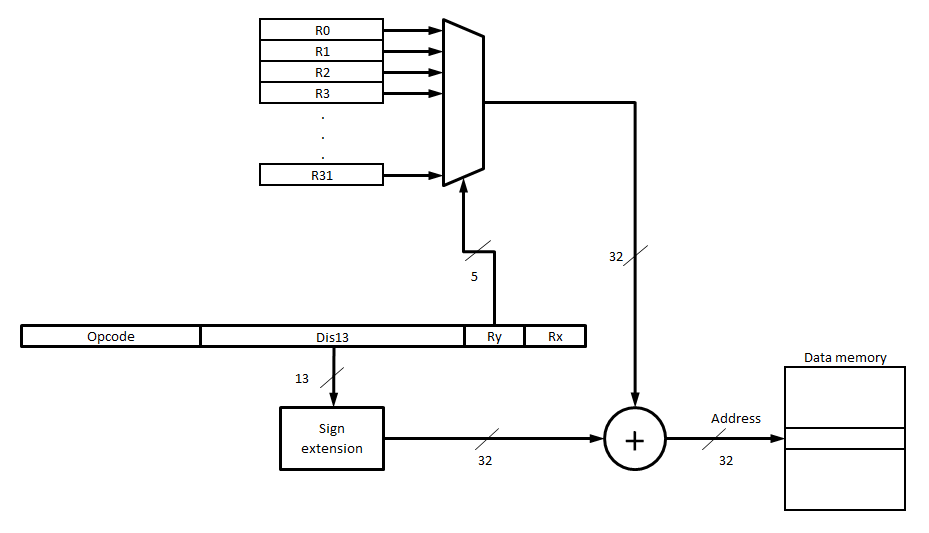
\includegraphics[scale=0.6]{./figures/eff_address.png}
\caption{Effective data memory address calculation.}
\end{figure}

\subsection{Instruction Memory}
\label{ssec:instruction_memory}

\begin{itemize}
   \item Instruction memory is read-only for the procesor. Read cycle takes only one clock period.
   \item Memory is organized in big-endian format.
   \item Only 32 bits single-word instructions are supported.
   \item An instruction can only be located in addresses multiple of 4.
   \item First 32 adresses (128 bytes) are reserved for exception vectors.
\end{itemize}
See figure \ref{fig:im_organization}

\begin{figure}
\begin{center}
\begin{bytefield}[bitwidth=0.9em]{40}
   \bitbox[]{8}{} & \bitbox[]{8}{+0} & \bitbox[]{8}{+1} & \bitbox[]{8}{+2} & \bitbox[]{8}{+3}\\
   \bitbox[]{8}{}
      & \bitbox[]{1}{\texttt{7}} & \bitbox[]{1}{\texttt{}} & \bitbox[]{1}{\texttt{}} & \bitbox[]{1}{\texttt{}}
      & \bitbox[]{1}{\texttt{}}  & \bitbox[]{1}{\texttt{}} & \bitbox[]{1}{\texttt{}} & \bitbox[]{1}{\texttt{0}}
      & \bitbox[]{1}{\texttt{7}} & \bitbox[]{1}{\texttt{}} & \bitbox[]{1}{\texttt{}} & \bitbox[]{1}{\texttt{}}
      & \bitbox[]{1}{\texttt{}}  & \bitbox[]{1}{\texttt{}} & \bitbox[]{1}{\texttt{}} & \bitbox[]{1}{\texttt{0}}
      & \bitbox[]{1}{\texttt{7}} & \bitbox[]{1}{\texttt{}} & \bitbox[]{1}{\texttt{}} & \bitbox[]{1}{\texttt{}}
      & \bitbox[]{1}{\texttt{}}  & \bitbox[]{1}{\texttt{}} & \bitbox[]{1}{\texttt{}} & \bitbox[]{1}{\texttt{0}}
      & \bitbox[]{1}{\texttt{7}} & \bitbox[]{1}{\texttt{}} & \bitbox[]{1}{\texttt{}} & \bitbox[]{1}{\texttt{}}
      & \bitbox[]{1}{\texttt{}}  & \bitbox[]{1}{\texttt{}} & \bitbox[]{1}{\texttt{}} & \bitbox[]{1}{\texttt{0}} \\
   \bitbox[]{8}{\texttt{0x00000000}} & \bitbox[ltb]{8}{Byte 3} & \bitbox[tb]{8}{Byte 2} & \bitbox[tb]{8}{Byte 1} & \bitbox[rtb]{8}{Byte 0}\\
   \bitbox[]{8}{\texttt{0x00000004}} & \bitbox[ltb]{8}{Byte 3} & \bitbox[tb]{8}{Byte 2} & \bitbox[tb]{8}{Byte 1} & \bitbox[rtb]{8}{Byte 0}\\
   \bitbox[]{8}{\texttt{0x00000008}} & \bitbox[ltb]{8}{Byte 3} & \bitbox[tb]{8}{Byte 2} & \bitbox[tb]{8}{Byte 1} & \bitbox[rtb]{8}{Byte 0}\\
   \bitbox[]{8}{\texttt{0x0000000C}} & \bitbox[ltb]{8}{Byte 3} & \bitbox[tb]{8}{Byte 2} & \bitbox[tb]{8}{Byte 1} & \bitbox[rtb]{8}{Byte 0}\\
   \bitbox[]{8}{}                    & \bitbox[lrt]{32}{} \\
   \bitbox[]{8}{}                    & \bitbox[lr]{32}{$\vdots$} \\
   \bitbox[]{8}{}                    & \bitbox[lrb]{32}{} \\
   \bitbox[]{8}{\texttt{0xFFFFFFFF}} & \bitbox[ltb]{8}{Byte 3} & \bitbox[tb]{8}{Byte 2} & \bitbox[tb]{8}{Byte 1} & \bitbox[rtb]{8}{Byte 0}\\
\end{bytefield}
\end{center}
\caption{Instruction memory organization.}
\label{fig:im_organization}
\end{figure}


\subsubsection{Program counter, branch and jump target addresses calculations}
\label{sssec:pc_branch_jump}
With instructions being 4 bytes long and unaligned access to instruction memory being not allowed, the effective instruction memory
address when stored in GPR's is given by bits 31 downto 2.
Branch or jump instructions that encode the address displacement in the corresponding field, also take advantage of this aligment
restriction, the two lower bits of the destination address are implicit (zeroes).

\subsection{Memory Timing Diagrams}
\label{ssec:memory_timing_diagrams}
\begin{figure}
\begin{center}
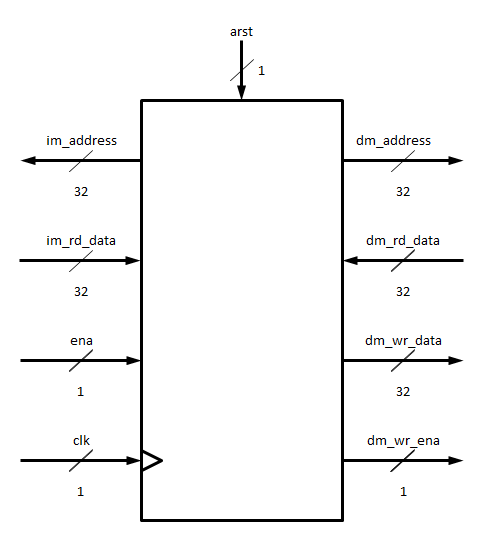
\includegraphics[scale=0.6]{./figures/interface.png}
\end{center}
\caption{Memory Port Interface.}
\label{fig:mem_port}
\end{figure}

\begin{figure}
\begin{center}
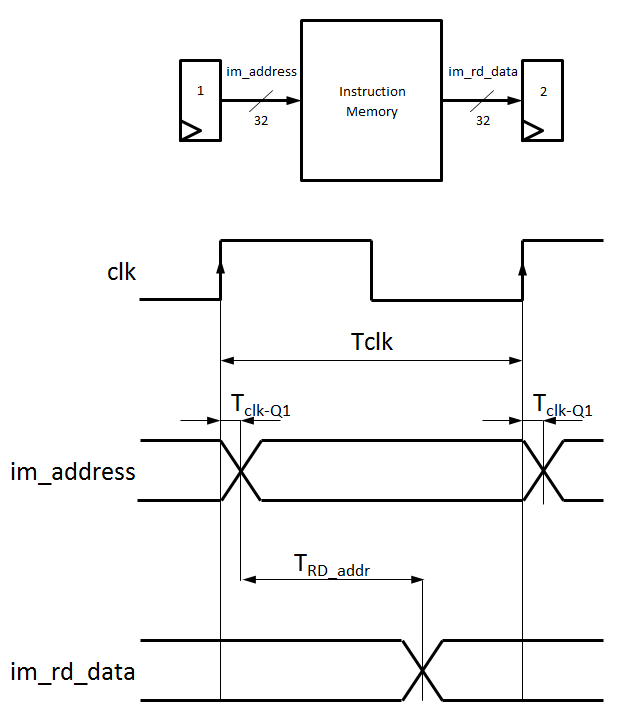
\includegraphics[scale=0.55]{./figures/im_rd_timing.png}
\end{center}
\caption{Instruction memory read cycle timing diagram.}
\label{fig:im_rd_timing}
\end{figure}

\begin{figure}
\begin{center}
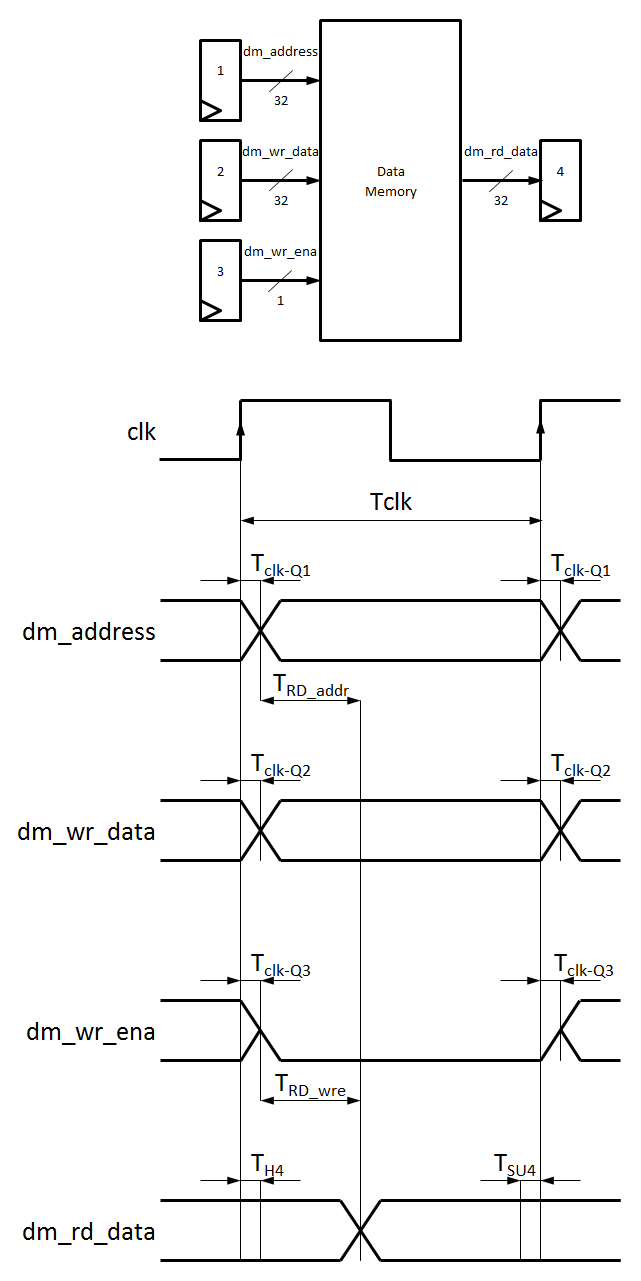
\includegraphics[scale=0.55]{./figures/dm_rd_timing.png}
\end{center}
\caption{Data memory read cycle timing diagram.}
\label{fig:dm_rd_timing}
\end{figure}

\begin{figure}
\begin{center}
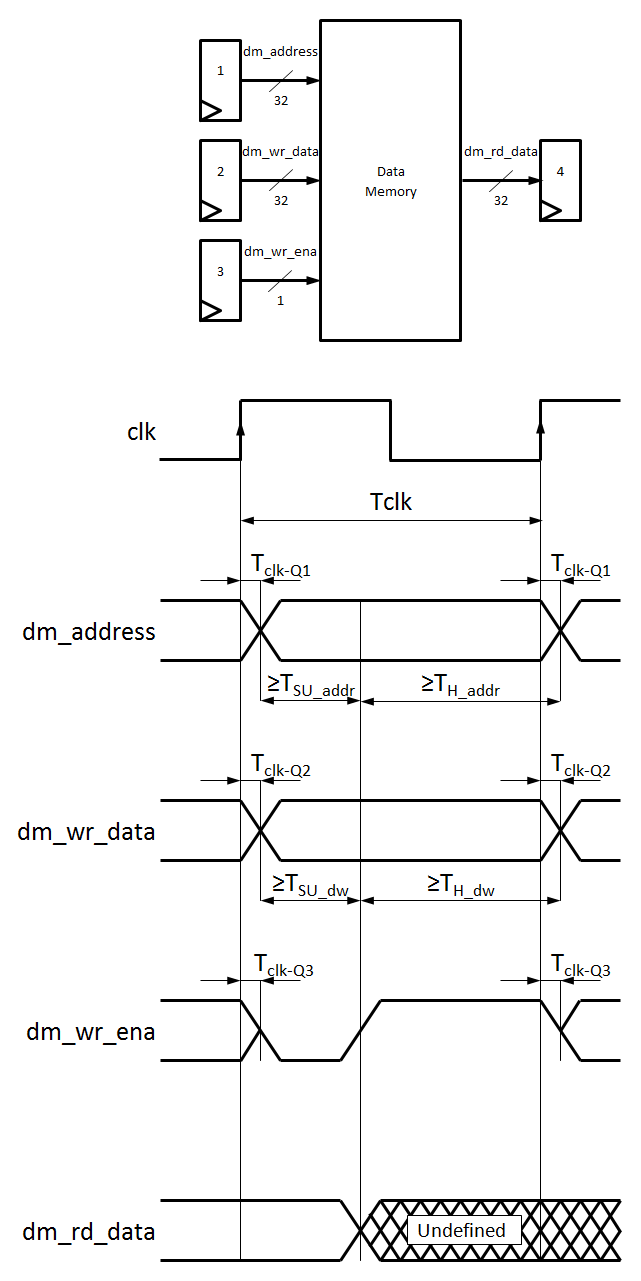
\includegraphics[scale=0.55]{./figures/dm_wr_timing.png}
\end{center}
\caption{Data memory write cycle timing diagram.}
\label{fig:dm_wr_timing}
\end{figure}

\begin{table}
\begin{center}
\begin{tabu} to \textwidth {|X[l]|X[l]|X[3,l]|}
\hline
\rowfont[c]\bfseries
\textbf{Parameter} & \textbf{Name} & \textbf{Description}\\
\hline
\hline
$T_{SU\_dw}$   & Write data setup time     & Minimum time to set dm\_wr\_data to a stable value before the rising edge of dr\_wr\_ena.\\
\hline
$T_{H\_dw}$    & Write data hold time      & Minimum time to hold dm\_wr\_data to a stable value after the rising edge of dr\_wr\_ena.\\
\hline
$T_{SU\_addr}$ & Address setup time        & Minimum time to set dm\_address to a stable value before the rising edge of dr\_wr\_ena.\\
\hline
$T_{H\_addr}$  & Address hold time         & Minimum time to hold dm\_address to a stable value after the rising edge of dr\_wr\_ena.\\
\hline
$T_{RD\_addr}$ & Read access time          & Maximum time taken by dm\_rd\_data to become valid after dm\_address changes.\\
\hline
$T_{RD\_wre}$  & Read access time          & Maximum time taken by dm\_rd\_data to become valid after dm\_wr\_ena goes low.\\
\hline
$T_{clk}$      & Clock period              & Period of time between two consecutive rising edges of clock signal.\\
\hline
$T_{clk-Q_i}$  & Clock to output time      & Propagation time of the register $i$.\\
\hline
$T_{SUi}$      & Register setup time       & Setup time of the register $i$.\\
\hline
$T_{Hi}$       & Register hold time        & Hold time of the register $i$.\\
\hline
\end{tabu}
\end{center}
\caption{Timing Parameters Description.}
\label{tbl:timing_paramerters}
\end{table}

\section{Execution of instruccions}

\subsection{The concept of `executing only if resources available'}
When decoded, a particular instruccion will only be executed if the resources used by the instruction are available.

Availability of resources means that source and destination operands and the corresponding execution unit are free
to perform the instruction execution. Otherwise, the instruction will be stalled till all resources are available.
This mechanism ensures that all instruction are always properly executed.

\subsection{ALU}
\textcolor{red}{Esto debería sacarse de acá}
The integer arithmetic logic unit (ALU) operates on 32 and 64 bits integer data sources and result. It also needs to
report carry, overflow, zero and negative flags. The ALU is in charge of all arithmetic and logic operations on GPR's.

\begin{table}
\begin{center}
\begin{tabu}{|X[l]|X[3,l]|X[c]|X[c]|}
\hline
\rowfont[c]\bfseries
Port name & Description & Size (Bits) & Type\\
\hline
\hline
clk                & Posedge active clock                         & 1  & Input   \\
\hline
start              & High active strobe start execution           & 1  & Input   \\
                   & Note: This signal must be implemented only for a non-pipelined ALU. & 1  & Input   \\
\hline
rst                & High active asynchronous reset               & 1  & Input   \\
\hline
srst               & High active synchronous reset                & 1  & Input   \\
\hline
ena		   & High active synchronous enable		  & 1  & Input \\
\hline
format             & Word or long word operands                   & 2  & Input   \\
                   & '0': Word                                    &    &         \\
                   & '1': Long                                    &    &         \\
\hline
operation          & Selects the operation to be executed         & XX & Input   \\
\hline
operand\_x         & First operand                                & 64 & Input   \\
\hline
operand\_y         & Second operand                               & 64 & Input   \\
\hline
flags              & Ouptut flags                                 & 3  & Output  \\
                   & Bit 0: zero                                  &    &         \\
                   & Bit 1: overflow                              &    &         \\
                   & Bit 2: carry                                 &    &         \\
                   & Note: Negative flag is implicit (MSB of the result) &    &         \\
\hline
result             & Operation result                             & 64 & Output  \\
\hline
done               & Up when finished and until start is asserted & 1  & Output  \\     
                   & Note: This signal must be implemented only for a non-pipelined ALU. & 1  & Input   \\
\hline
\end{tabu}
\end{center}
\caption{ALU Port interface}
\label{tbl:alu_interface}
\end{table}

\subsection{Floating point unit}
\textcolor{red}{Esto debería sacarse de acá}
The floating point unit (FPU) is optional to the design. The FPU is in charge of all arithmetic and logic operations on FPR's
operating on 32 and 64 bits formats.

When FPU is not provided, floating point operations must always generate
an exception and the corresponding exception mask should not be set. In this case, software support must be provided to handle the
exception and returning a consistent result, so the execution of the program can be resumed. Read section \ref{sec:exceptions} for more
information.

If the optional FPU is present, it must be IEEE 754 compliant and provide the following interface.

\begin{table}
\begin{center}
\begin{tabu}{|X[l]|X[3,l]|X[c]|X[c]|}
\hline
\rowfont[c]\bfseries
Port name & Description & Size (Bits) & Type\\
\hline
\hline
clk                & Posedge active clock                         & 1  & Input   \\
\hline
start              & High active strobe start execution           & 1  & Input   \\
                   & Note: This signal must be implemented only for a non-pipelined FPU. & 1  & Input   \\
\hline
rst                & High active asynchronous reset               & 1  & Input   \\
\hline
srst               & High active synchronous reset                & 1  & Input   \\
\hline
ena		   & High active synchronous enable		  & 1  & Input \\
\hline
fp\_format         & Single or double precission operands         & 2  & Input   \\
                   & '0': Single                                  &    &         \\
                   & '1': Double                                  &    &         \\
\hline
rnd\_mode          & Establishes rounding mode for the result     & 2  & Input   \\
                   & '00': RN - Round to nearest                  &    &         \\
                   & '01': RZ - Round towards zero                &    &         \\
                   & '10': RP - Round towards plus infinity       &    &         \\
                   & '11': RM - Round towards minus infinity      &    &         \\
\hline
operation          & Selects the operation to be executed         & XX & Input   \\
\hline
operand\_x         & First operand                                & 64 & Input   \\
\hline
operand\_y         & Second operand                               & 64 & Input   \\
\hline
cause              & Exception cause                              & 4  & Output  \\
                   & Bit 0: Underflow                             &    &         \\
                   & Bit 1: Overflow                              &    &         \\
                   & Bit 2: Division by zero                      &    &         \\
                   & Bit 3: Invalid operation                     &    &         \\
\hline
flags              & Ouptut flags                                 & 3  & Output  \\
                   & Bit 0: Zero                                  &    &         \\
                   & Bit 1: Infinity                              &    &         \\
                   & Bit 2: A number                              &    &         \\
                   & Note: Negative flag is implicit (MSB of the result) &    &         \\
\hline
result             & Operation result                             & 64 & Output  \\
\hline
done               & Up when finished and until start is asserted & 1  & Output  \\
                   & Note: This signal must be implemented only for a non-pipelined FPU. & 1  & Input   \\
\hline
\end{tabu}
\end{center}
\caption{ALU Port interface}
\label{tbl:fpu_interface}
\end{table}

\subsection{FPU timig diagrams}
\begin{figure}
\begin{center}
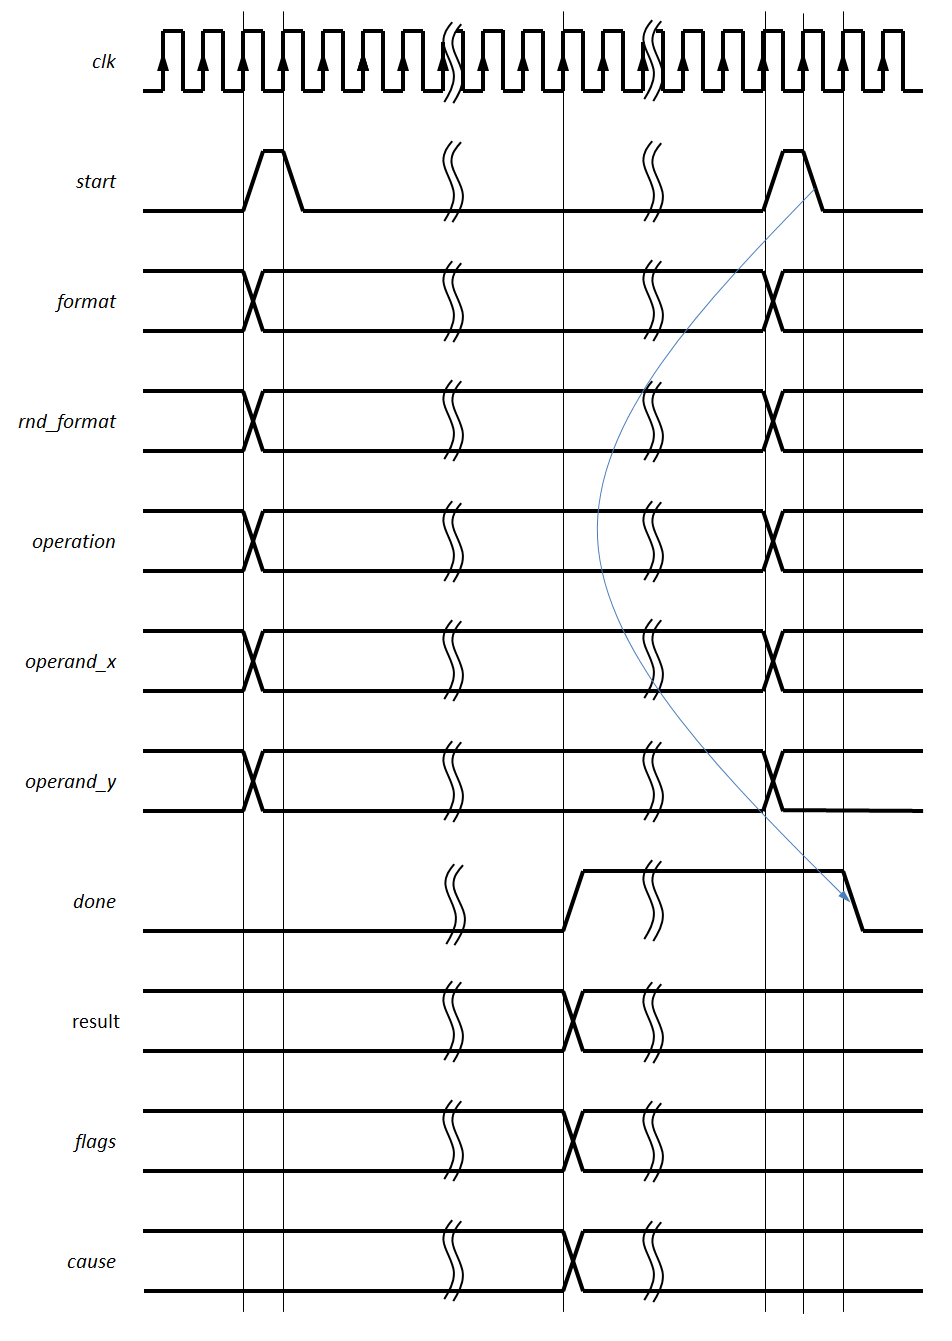
\includegraphics[scale=0.35]{./figures/fpu_timing.png}
\end{center}
\caption{FPU timing diagram.}
\label{fig:fpu_timing}
\end{figure}

\section{Exceptions}
\label{sec:exceptions}
Exceptions are handled by raising a flag, the offending (or interrupted) instruction address + 1 is stored in an L register.
When an exception condition is detected, the PC is loaded with the indexed special address $idx$ (exception identification immediate).
Reset is treated just as another source of exception.
Being the CR 32 bits wide, the architecture provides a space of 32 different
sources of exceptions, so the first 32 instruction addresses (from 0x00000000 to 0x0000007C) are reserved for exception handlers.\\
Exceptions should only be handled if the correspondig bit in MR is unset. As stated in section \ref{sec:registers}, MR has 33 physical
bits. The higher bit is a global mask for all exceptions and it is a hardware mechanism to avoid nested exceptions
when they are disabled.\\
Interrupts are handled as exceptions. Instructions stored at the special addresses must provide the handling for the exceptions.
Priorities are fixed and they correspond with the order stated in the listing below. Lower ordered exceptions always have higher priority over other
sources of exceptions.\\
The lowest priority is software generated exceptions (\emph{trap} instruction); thus it has the highest number, 31. On the other end, reset has the highest priority
(and the lowest number, 0).\\
The indexed address schema provides space for one instruction to start the handling routine.\\
Sources of exception not defined in this document are left free for future revisions of the architecture or implementation specific
exceptions.

\begin{itemize}
\item E0: Reset
\item E1: System tick.
\item E2: Execute invalid instruction.
\item E3: Misaligned data memory access.
\item E4: Misaligned long GPR access.
\item E5: Misaligned double FPR access.
\item E6: Integer division by zero.
\item E7: Long integer division by zero.
\item E8: Instruction is a FPU operation.
\item E9: Instruction is a FPU extendended operation.
\item E10: FPU\_V flag is set.
\item E11: FPU\_Z flag is set.
\item E12: FPU\_O flag is set.
\item E13: FPU\_U flag is set.
\item E30: Interruption request.
\item E31: Trap.
\end{itemize}

Nested exceptions support is configured by means of the bit 1 of the CFG register. If not supported, the CPU cannot
accept a new source of exception until the handling of the current one has finished. On the other hand, when
nested interruptions are supported, only a higher priority exception can interrupt the current one.\\

\subsection{Exception handling}
\label{ssec:exception_handling}
As stated earlier, the nested exception support can be enabled/disabled through the bit 1 of the CFG register.

\subsubsection{Nested insterruptions disabled}
\label{sssec:nested_irq_disabled}
In table \ref{tbl:nid_steps} interruption handling with nested interruptions disabled is described; pc is the offending (or interrupted) instruction address.

\begin{table}
\begin{center}
\begin{tabu} to \textwidth {|X[r]|X[2,l]|X[l]|X[2,l]|}
\rowfont[c]\bfseries
\hline
Step & Description & Assembly & Registers Status\\
\hline
\hline
1. & Exception $idx$ is raised             &                  & if $(mr[idx]==`0')$ then \\
   &                                       &                  & \hspace{20pt}$l_0[29:0] \leftarrow_{30} (pc + 1)$ \\
   &                                       &                  & \hspace{20pt}$pc \leftarrow_{30} idx$ \\
   &                                       &                  & \hspace{20pt}$mr[32] \leftarrow_{1} 1$ \\
   &                                       &                  & \hspace{20pt}$cr[idx] \leftarrow_{1} 0$ \\
   &                                       &                  & \hspace{20pt}$cfg[0] \leftarrow_{1} 0$ \\
   &                                       &                  & \hspace{20pt}continue with step 2.\\
   &                                       &                  & else\\
   &                                       &                  & \hspace{20pt}Do not handle the exception \\
   &                                       &                  & endif \\
\hline
2. & Jump to the exception handler routine & \texttt{j dis26} & $pc \leftarrow_{30} pc + sx_{30}(dis26)$ \\
\hline
3. & Save context to be used in handler    & User code        & \\
\hline
4. & Handler routine                       & User code        & \\
\hline
5. & Recover context                       & User code        & \\
\hline
6. & Return from exception                 & \texttt{rfe}     & $pc \leftarrow_{30} l_0[29:0]$ \\
   &                                       &                  & $mr[32] \leftarrow_{1} 0$ \\
   &                                       &                  & $cfg[0] \leftarrow_{1} 1$ \\
\hline
\end{tabu}
\end{center}
\caption{Nested Interruptions Disabled Interrupt Sequence}
\label{tbl:nid_steps}
\end{table}


\subsubsection{Nested insterruptions enabled}
\label{sssec:nested_irq_enabled}
In table \ref{tbl:nie_steps} interruption handling with nested interruptions disabled is described; pc is the offending (or interrupted) instruction address.

\begin{table}
\begin{center}
\begin{tabu} to \textwidth {|X[r]|X[2,l]|X[l]|X[2,l]|}
\rowfont[c]\bfseries
\hline
Step & Description & Assembly & Registers Status\\
\hline
\hline
1. & Exception $idx$ is raised             &                  & if $(mr[idx]==`0')$ \&\& $(idx < l_{esp}[35:30])$ then \\
   &                                       &                  & \hspace{20pt}$l_{esp}[29:0] \leftarrow_{30} (pc + 1)$ \\
   &                                       &                  & \hspace{20pt}$esp \leftarrow_{5} (esp + 1)$ \\
   &                                       &                  & \hspace{20pt}$l_{esp}[34:30] \leftarrow_{5} idx$ \\
   &                                       &                  & \hspace{20pt}$pc \leftarrow_{30} idx$ \\
   &                                       &                  & \hspace{20pt}$cr[idx] \leftarrow_{1} 0$ \\
   &                                       &                  & \hspace{20pt}$cfg[0] \leftarrow_{1} 0$ \\
   &                                       &                  & \hspace{20pt}continue with step 2.\\
   &                                       &                  & else\\
   &                                       &                  & \hspace{20pt}Do not handle the exception \\
   &                                       &                  & endif \\
\hline
2. & Jump to the exception handler routine & \texttt{j dis26} & $pc \leftarrow_{30} pc + sx_{30}(dis26)$ \\
\hline
3. & Save context to be used in handler    & User code        & \\
\hline
4. & Handler routine                       & User code        & \\
\hline
5. & Recover context                       & User code        & \\
\hline
6. & Return from exception                 & \texttt{rfe}     & $esp \leftarrow_{5} esp - 1$ \\
   &                                       &                  & $pc \leftarrow_{30} l_{esp}[29:0]$ \\
   &                                       &                  & $cfg[0] \leftarrow_{1} 1$ \\

\hline
\end{tabu}
\end{center}
\caption{Nested Interruptions Enabled Sequence Detail}
\label{tbl:nie_steps}
\end{table}

\subsection{Reset exception}
\label{ssec:reset_exception}
As stated before, reset is just another exception, but there are a few differences with the other sources.\\
The reset exception cannot be masked: altough MR can be written with the lower bit set, the reset exception will not be masked. Also,
it will not be masked by the global mask bit, enabling the reset to happen even if an exception is being handled.\\

\subsubsection{Getting out of the reset exception and booting}
The reset mechanism will set all registers with zero (except L0), though, the first instruction
excecuted by the microprocesor is in address \texttt{0x00000000}, and as the CFG register is zeroed, the microprocesor will run in supervisor mode.
Thus, the reset address is the vectored address for the reset exception. That instruction should be a jump to the reset exception handler. This
handler should implement all the boot code necessary to set up the environment. As L0[29:0] is loaded with 0 (as a consequence of
the reset) the code cannot call $rfe$ to get out of the exception (calling $rfe$ will load the PC with the reset address again). So CFG
register must be manually set to user mode once initialization is done and everything is ready to start running user code via
a \emph{movi2s} instruction.

\subsection{System tick}
\label{ssec:sys_tick}
System tick is a periodic exception internally generated by the CPU hardware.The system timer is a 32 bits down counter that
generates the systick exception when reaches zero. The reload value of the system timer can be configured trough
the STP register.

The CFG register (bit 2) sets the system timer behavior. If unset, the timer will be in free running mode, meaning that
once the timer reaches zero, it will be automatically reloaded with the value $(1024*STP) + 1023$ and will continue counting down.
On the other hand, if set, the system timer will stop when reaches zero and will reload the value $(1024*STP) + 1023$ and
resume the count down after CFG[3] is written with \emph{movi2s}.

The bit 3 of the CFG register is not persistent, it means that goes back to '0' one clock cycle after it was written.
Always returns '0' on read.

\subsection{Interruptions}
The CPU is hardware interrupted by rising the interrupt input port (\emph{irq}) and exception E30 is launched if not masked.
When the processor attends the interruption exception, the $iack$ output is raised by the processor indicating
that the exception was already handled. The $iack$ output is set low by the CPU when a new interruption request occurs. Fig.
\ref{fig:int_sequence} shows a timing diagram of the interruption sequence.

\begin{figure}
\begin{center}
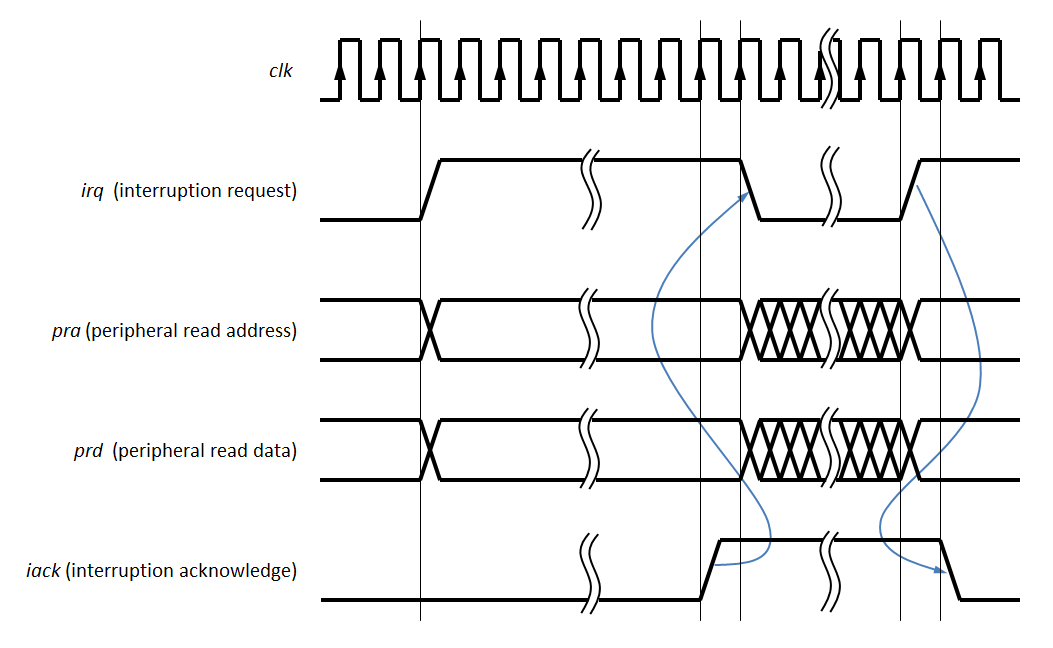
\includegraphics[scale=0.55]{./figures/int_td.png}
\caption{Interruption timing diagram.}
\label{fig:int_sequence}
\end{center}
\end{figure}




\section{Operating modes}
\label{sec:modes}
The processor has two different operating modes: \emph{supervisor mode}
and \emph{user mode}.

In supervisor mode, all instructions can be executed and the CFG[0]
register is unset.

In user mode, some instructions can not be executed. Any attempt to execute
one of those instructions causes an invalid operation exception (E2). The user
mode is indicated by setting CFG[0].

The privileged instructions (those that can only be executed in supervisor mode)
are the following:

\begin{itemize}
\item \texttt{movi2s}
\item \texttt{movs2i}
\item \texttt{rfe}
\end{itemize}

The reset mode is always supervisor mode.

The instruction \emph{trap} is used by user programs to generate software exceptions (providing a mechanism to implement system calls).

The \emph{rfe} returns the processor to user mode. Another way to return the processor
to user mode is by setting CFG[0].

\section{Peripherals}
\label{sec:peripherals}
Comunication with peripherals is achieved through interruptions and four special porpouse registers: PWD, PRD, PWA, and PRA.

Whenever a peripheral should be written the sequence that must be followed is:
\begin{itemize}
 \item PWA must be set using \emph{movi2s} with the peripheral address.
 \item PWD must be set using \emph{movi2s} instruction to copy the information from one of the GPR's. Automatically,
       a strobe is generated on the \emph{pwd\_wr\_ena} output pin signaling the writting operation.
\end{itemize}

Whenever a peripheral should be read the sequence that must be followed is:
\begin{itemize}
 \item PRA must be set by external hardware.
 \item PRD must be set by external hardware.
 \item The \emph{irq} line is raised.
\end{itemize}
Since the system is synchronous with the CPU clock, the three events avobe can happen at the same time (i.e. in the
same clock cycle).


% \chapter{Application binary interface}
% The appication binary interface (ABI) covers details such as:
\begin{itemize}
\item The sizes, layout, and alignment of data types.
\item The calling convention, which controls how functions' arguments are passed and return values retrieved;
for example, whether all parameters are passed on the stack or some are passed in registers, which registers
are used for which function parameters, and whether the first function parameter passed on the stack is pushed
first or last onto the stack.
\item How an application should make system calls to the operating system.
\item The binary format of object files and program libraries.
\end{itemize}

This description is focused on ISO/IEC 9899:1990 C language support.

\section{Scalar data types}

\begin{table}
  \begin{center}
    \begin{tabular}{|c|c|c|c|}
    \hline
    \textbf{C language type} & \textbf{Size of [bytes]} & \textbf{Aligment [bytes]} & \textbf{CPU equivalent}\\
    \hline
    \hline
    char                   & 1  & 1 & byte \\
    \hline
    unsigned char          & 1  & 1 & byte \\
    \hline
    short int              & 2  & 2 & half \\
    \hline
    unsigned short int     & 2  & 2 & half \\
    \hline
    int                    & 4  & 4 & word \\
    \hline
    unsigned int           & 4  & 4 & word \\
    \hline
    long int               & 8  & 4 & double word \\
    \hline
    unsigned long int      & 8  & 4 & double word \\
    \hline
    long long int          & 8  & 4 & double word  \\
    \hline
    unsigned long long int & 8  & 4 & double word  \\
    \hline
    float                  & 4  & 4 & float \\
    \hline
    double                 & 8  & 4 & double \\
    \hline
    long double            & 8  & 4 & double \\
    \hline
    pointer (any type)     & 4  & 4 & word \\
    \hline
    \end{tabular}
  \caption{Data types equivalence.}
  \label{tbl:abi_data_types}
  \end{center}
\end{table}
A null pointer of any type must be zero.


\subsection{Aggregates and Unions}
Aggregates (structures and arrays) and unions assume the alignment of their most strictly aligned element.
\begin{itemize}
\item An array uses the alignment of its elements.
\item Structures and unions, since their elements may be of different types, can require padding to meet alignment restrictions.
      Each element is assigned to the lowest aligned address.
\end{itemize}














\subsection{System calls}
\label{sec:system_calls}
In the following description \emph{ids} is system call ID.


xxxxxxxxx mejorar esto para cuando soporta y no soporta nested exceptions xxxxxxxxxxxxxx

\begin{center}
\begin{tabular}{|r|l|l|l|}
\hline
\textbf{Step} & \textbf{Description} & \textbf{Assembly} & \textbf{Registers Status}\\
\hline
\hline
1. & System call ID (\emph{ids}) is saved in rx & \texttt{        movi rx, ids}    & \hspace{20pt}$rx \leftarrow_{32} ids$ \\
\hline
2. & Jump to the exception handler routine      & \texttt{        trap}            & \hspace{20pt}$l_{esp}[29:0] \leftarrow_{30} pc + 1$ \\
   &                                            &                                  & \hspace{20pt}$pc \leftarrow_{30} 31$ \\
\hline
3. & Jump                                       & \texttt{    31: jump \$trap}     & \hspace{20pt}$pc \leftarrow_{30} trap$ \\
\hline
4. & Jump to system call routine                & \texttt{\$trap: jr rx}           & \hspace{20pt}$pc \leftarrow_{30} pc + ids$ \\
\hline
5. & System call routine                        & System call code                 & \\
\hline
6. & Return from system call                    & \texttt{rfe}                     & $pc \leftarrow_{30} l_{esp}[29:0]$ \\
   &                                            &                                  & $mr[32] \leftarrow_{1} 0$ \\
   &                                            &                                  & $cfg[0] \leftarrow_{1} 1$ \\
\hline
\end{tabular}
\end{center}



\subsection{Subroutine calls}
\label{sec:subroutine_calls}
In the following description \emph{idr} is subroutine ID.

\begin{center}
\begin{tabular}{|r|l|l|l|}
\hline
\textbf{Step} & \textbf{Description} & \textbf{Assembly} & \textbf{Registers Status}\\
\hline
\hline
1. & Subroutine call ID (\emph{idr}) is saved in rx & \texttt{ jal rx, idr}            & \hspace{20pt}$rx \leftarrow_{32} pc+1$ \\
   &                                                &                                  & \hspace{20pt}$pc \leftarrow_{30} pc + idr$ \\
\hline
3. & Subroutine                                     & User code                        & \\
\hline
6. & Return from subroutine                         & \texttt{jr rx}                   & $pc \leftarrow_{30} rx[29:0]$ \\
\hline
\end{tabular}
\end{center}
















\chapter{Detailed instruction set description}
% Cargar CSV con ISA
\DTLsetseparator{|}
\DTLloaddb[]{isa}{latex/isa/isa.csv}
% \DTLloadrawdb[]{isa}{latex/isa/isa.ddb}

\section{Instruction Set Architecture}
\label{sec:isa}

\subsection{Instruction format}
\label{ssec:instruction_format}
There are four intruction main types according to how many registers are used as arguments of the instruction, named Type 0, 1, 2 and 3. The type of
instruction is identified by the two most significant bits of the opcode. This types of instructions are further organized in groups, which identify if
the registers are used as sources or destinations and the role of the remaining bits of the opcode, such as immediate data, displacement, subopcodes or
size of the operation (width of the affected data).

\subsubsection{Type 0 instructions}
\label{sssec:type_0}
Type 0 instructions are encoded with only two bits (bits 28 and 29). Usage of the 28 remaining bits depend on the instruction itself. This type of
instructions are further divided in two groups: A and B. Group A has a 28 bit displacement field. Group B does not specify those bits. The enconding
structure is shown in figure \ref{fig:type_0_encoding_structure}.

\begin{figure}
  \begin{center}
    \begin{bytefield}[endianness=big,bitwidth=0.9em]{40}
       \bitbox[]{8}{Group} & \bitbox[]{32}{Encoding Structure}\\
       \bitbox[]{40}{}\\
       
       \bitbox[]{8}{} & \bitbox[]{2}{2} & \bitbox[]{2}{2} & \bitbox[]{28}{28 bits}\\
       \bitheader{0-31}\\
       \bitbox[]{8}{Group A} & \bitbox{2}{T} & \bitbox{2}{O} & \bitbox{28}{Displacement}\\
       
       \bitbox[]{40}{}\\
       
       \bitbox[]{8}{} & \bitbox[]{2}{2} & \bitbox[]{2}{2} & \bitbox[]{28}{28 bits}\\
       \bitheader{0-31}\\
       \bitbox[]{8}{Group B} & \bitbox{2}{T} & \bitbox{2}{O} & \bitbox{28}{Undefined}\\
    \end{bytefield}
  \end{center}
  \caption{Type 0 instruction encoding structure}
  \label{fig:type_0_encoding_structure}
\end{figure}

\subsubsection{Type 1 instructions}
\label{sssec:type_1}
Type 1 instructions are encoded with four bits (bits 26 to 29) and make use of one register, either as source or destination of the operation. This type
of instructions is further divided in four groups: A, B, C and D. Group A uses a source register (addressed by bits 21 to 25) and a twenty one bits
displacement field (bits 0 to 20). Group B uses a destination register (addressed by bits 16 to 20) and a 16 bits displacement field (bits 0 to 15),
leaving 5 bits unespecified (bits 21 to 25). Group C uses a source register (addressed by bits 21 to 25), a 4 bits subopcode (bits 17 to 20) and a 17 bits
displacement field (bits 0 to 16). Group D uses a destination register (addressed by bits 16 to 20) and a 16 bits immediate field (bits 0 to 15), leaving 5
bits unespecified (bits 21 to 25). The encoding structure is shown in figure \ref{fig:type_1_encoding_structure}.

\begin{figure}
  \begin{center}
    \begin{bytefield}[endianness=big,bitwidth=0.9em]{40}
       \bitbox[]{8}{Group} & \bitbox[]{32}{Encoding Structure}\\
       \bitbox[]{40}{}\\
       
       \bitbox[]{8}{} & \bitbox[]{2}{2} & \bitbox[]{4}{4 bits} & \bitbox[]{5}{5 bits} & \bitbox[]{21}{21 bits}\\
       \bitheader{0-31}\\
       \bitbox[]{8}{Group A} & \bitbox{2}{T} & \bitbox{4}{Opcode} & \bitbox{5}{R src} & \bitbox{21}{Displacement}\\
       
       \bitbox[]{40}{}\\
       
       \bitbox[]{8}{} & \bitbox[]{2}{2} & \bitbox[]{4}{4 bits} & \bitbox[]{5}{5 bits} & \bitbox[]{5}{5 bits} & \bitbox[]{16}{16 bits}\\
       \bitheader{0-31}\\
       \bitbox[]{8}{Group B} & \bitbox{2}{T} & \bitbox{4}{Opcode} & \bitbox{5}{Undefined} & \bitbox{5}{R dst} & \bitbox{16}{Displacement}\\
       
       \bitbox[]{40}{}\\
       
       \bitbox[]{8}{} & \bitbox[]{2}{2} & \bitbox[]{4}{4 bits} & \bitbox[]{5}{5 bits} & \bitbox[]{4}{4 bits} & \bitbox[]{17}{17 bits}\\
       \bitheader{0-31}\\
       \bitbox[]{8}{Group C} & \bitbox{2}{T} & \bitbox{4}{Opcode} & \bitbox{5}{R src} & \bitbox{4}{Sub Op} & \bitbox{17}{Displacement}\\
       
       \bitbox[]{40}{}\\
       
       \bitbox[]{8}{} & \bitbox[]{2}{2} & \bitbox[]{4}{4 bits} & \bitbox[]{5}{5 bits} & \bitbox[]{5}{5 bits} & \bitbox[]{16}{16 bits}\\
       \bitheader{0-31}\\
       \bitbox[]{8}{Group D} & \bitbox{2}{T} & \bitbox{4}{Opcode} & \bitbox{5}{Undefined} & \bitbox{5}{R dst} & \bitbox{16}{Immediate}\\
    \end{bytefield}
  \end{center}
  \caption{Type 1 instruction encoding structure}
  \label{fig:type_1_encoding_structure}
\end{figure}

\subsubsection{Type 2 instructions}
\label{sssec:type_2}
Type 2 instructions are encoded with four bits (bits 26 to 29) and make use of two registers, one being always source and the other one either source or
destination of the operation. This type of instructions are further divided in five groups: A, B, C, D and E. Group A uses a source register (bits 21 to
25), a destination register (bits 16 to 20), a 5 bits subopcode (bits 4 to 8), a 2 bits variation specifier (bits 9 and 10), leaving 9 bits unespecified
(bits 0 to 3 and 11 to 15). Group B uses a source register (bits 21 to 25), a destination register (bits 16 to 20) and a 16 bits displacement field (bits 0
to 15). Group C uses a source register (bits 21 to 25), a destination register (bits 16 to 20) and a 16 bits immediate field (bits 0 to 15). Group D uses
two source registers (bits 21 to 25 and 16 to 20) and a 16 bits displacement field (bits 0 to 15). Group E uses a source register (bits 21 to 25), a
destination register (bits 16 to 20), a two bits subopcode field (bits 14 and 15), a three bits data field (bits 11 to 13), leaving 11 bits unespecified
(bits 0 to 10). The encoding structure is shown in figure \ref{fig:type_2_encoding_structure}.

\begin{figure}
  \begin{center}
    \begin{bytefield}[endianness=big,bitwidth=0.9em]{40}
       \bitbox[]{8}{Group} & \bitbox[]{32}{Encoding Structure}\\
       \bitbox[]{40}{}\\
       
       \bitbox[]{8}{} & \bitbox[]{2}{2} & \bitbox[]{4}{4 bits} & \bitbox[]{5}{5 bits} & \bitbox[]{5}{5 bits} & \bitbox[]{5}{5 bits} & \bitbox[]{2}{2} & \bitbox[]{5}{5 bits} & \bitbox[]{4}{4 bits}\\
       \bitheader{0-31}\\
       \bitbox[]{8}{Group A} & \bitbox{2}{T} & \bitbox{4}{Opcode} & \bitbox{5}{R src} & \bitbox{5}{R dst} & \bitbox{5}{Undefined} & \bitbox{2}{V} & \bitbox{5}{Sub Op} & \bitbox{4}{Undef}\\
       
       \bitbox[]{40}{}\\
       
       \bitbox[]{8}{} & \bitbox[]{2}{2} & \bitbox[]{4}{4 bits} & \bitbox[]{5}{5 bits} & \bitbox[]{5}{5 bits} & \bitbox[]{16}{16 bits}\\
       \bitheader{0-31}\\
       \bitbox[]{8}{Group B} & \bitbox{2}{T} & \bitbox{4}{Opcode} & \bitbox{5}{R src} & \bitbox{5}{R dst} & \bitbox{16}{Displacement}\\
       
       \bitbox[]{40}{}\\
       
       \bitbox[]{8}{} & \bitbox[]{2}{2} & \bitbox[]{4}{4 bits} & \bitbox[]{5}{5 bits} & \bitbox[]{5}{5 bits} & \bitbox[]{16}{16 bits}\\
       \bitheader{0-31}\\
       \bitbox[]{8}{Group C} & \bitbox{2}{T} & \bitbox{4}{Opcode} & \bitbox{5}{R src} & \bitbox{5}{R dst} & \bitbox{16}{Immediate}\\
       
       \bitbox[]{40}{}\\
       
       \bitbox[]{8}{} & \bitbox[]{2}{2} & \bitbox[]{4}{4 bits} & \bitbox[]{5}{5 bits} & \bitbox[]{5}{5 bits} & \bitbox[]{16}{16 bits}\\
       \bitheader{0-31}\\
       \bitbox[]{8}{Group D} & \bitbox{2}{T} & \bitbox{4}{Opcode} & \bitbox{5}{R src 1} & \bitbox{5}{R src 2} & \bitbox{16}{Displacement}\\
       
       \bitbox[]{40}{}\\
       
       \bitbox[]{8}{} & \bitbox[]{2}{2} & \bitbox[]{4}{4 bits} & \bitbox[]{5}{5 bits} & \bitbox[]{5}{5 bits} & \bitbox[]{2}{2} & \bitbox[]{3}{3 bits} & \bitbox[]{11}{11 bits}\\
       \bitheader{0-31}\\
       \bitbox[]{8}{Group E} & \bitbox{2}{T} & \bitbox{4}{Opcode} & \bitbox{5}{R src} & \bitbox{5}{R dst} & \bitbox{2}{SO} & \bitbox{3}{Nib} & \bitbox{11}{Undefined}\\
    \end{bytefield}
  \end{center}
  \caption{Type 2 instruction encoding structure}
  \label{fig:type_2_encoding_structure}
\end{figure}

\subsubsection{Type 3 instructions}
\label{sssec:type_3}
Type 3 instructions make use of three registers, two sources and one destination. This type of instructions are not further divided in groups. All three 
registers are encoded with five bits each (bits 21 to 25 and bits 11 to 15 for source registers and bits 16 to 20 for destination register), a 5 bits
subopcode field (bits 4 to 8), a 2 bits variation specifier (bits 9 and 10), leaving 8 bits undefined (bits 0 to 3 and 26 to 29). The encoding structure is
shown in figure \ref{fig:type_3_encoding_structure}.

\begin{figure}
  \begin{center}
    \begin{bytefield}[endianness=big,bitwidth=0.9em]{40}
       \bitbox[]{8}{Group} & \bitbox[]{32}{Encoding Structure}\\
       \bitbox[]{40}{}\\
       
       \bitbox[]{8}{} & \bitbox[]{2}{2} & \bitbox[]{4}{4 bits} & \bitbox[]{5}{5 bits} & \bitbox[]{5}{5 bits} & \bitbox[]{5}{5 bits} & \bitbox[]{2}{2} & \bitbox[]{5}{5 bits} & \bitbox[]{4}{4 bits}\\
       \bitheader{0-31}\\
       \bitbox[]{8}{All} & \bitbox{2}{T} & \bitbox{4}{Undef} & \bitbox{5}{R src 1} & \bitbox{5}{R dst} & \bitbox{5}{R src 2} & \bitbox{2}{V} & \bitbox{5}{Sub Op} & \bitbox{4}{Undef}\\
    \end{bytefield}
  \end{center}
  \caption{Type 3 instruction encoding structure}
  \label{fig:type_3_encoding_structure}
\end{figure}

\subsection{Full instruction set}
\label{ssec:full_isa}

\subsubsection{Arranged by type}
\label{sssec:isa_by_type}

This sections tabulates instructions organized by type.\\
\begin{itemize}
  \item Type 0 instructions are summarized in table \ref{tbl:type_0}.
  \item Type 1 instructions are summarized in table \ref{tbl:type_1}.
  \item Type 2 instructions are summarized in table \ref{tbl:type_2}.
  \item Type 3 instructions are summarized in table \ref{tbl:type_3}.
\end{itemize}

\begin{table}
  \begin{center}
    \begin{tabu} to \textwidth {llX[l]}
      \hline
      \multicolumn{2}{c}{Mnemonic} & Description \\
      \DTLforeach*[\DTLiseq{\type}{0} \and \DTLiseq{\group}{A}]
        {isa}
	{
	  \mnemonic=mnemonic,
	  \args=args,
	  \shortdescription=shortdescription,
	  \type=type,
	  \group=group}
	{
	  \DTLiffirstrow{\\\hline\hline}{\\} \texttt{\mnemonic} & \texttt{\args} & \shortdescription
	}
      \DTLforeach*[\DTLiseq{\type}{0} \and \DTLiseq{\group}{B}]
        {isa}
	{
	  \mnemonic=mnemonic,
	  \args=args,
	  \shortdescription=shortdescription,
	  \type=type,
	  \group=group}
	{
	  \DTLiffirstrow{\\\hline}{\\} \texttt{\mnemonic} & \texttt{\args} & \shortdescription
	} \\\hline
    \end{tabu}
  \end{center}
\end{table}

\subsubsection{Arranged by function}
\label{sssec:isa_by_function}
This section further tabulates instructions according to their functional behavior, listed as follows:

\begin{itemize}
  \item Register data transfer are summarized in table \ref{tbl:register_data_transfer_instructions}.
  \item Memory data transfer are summarized in table \ref{tbl:memory_data_transfer_instructions}.
  \item Arithmetic are summarized in table \ref{tbl:arithmetic_instructions}.
  \item Cordic are summarized in table \ref{tbl:cordic_instructions}.
  \item Logic are summarized in table \ref{tbl:logic_instructions}.
  \item Control are summarized in table \ref{tbl:control_instructions}.
  \item Data are summarized type conversion in table \ref{tbl:data_type_conversion_instructions}.
\end{itemize}

\begin{table}
  \begin{center}
    \begin{tabu} to \textwidth {|ll|X[l]|}
      \hline
      \multicolumn{2}{|c|}{Mnemonic} & Description
      \DTLforeach*[\DTLiseq{\family}{Register data transfer} \and \DTLiseq{\subfamily}{0}]
	{isa}
	{
	  \mnemonic=mnemonic,
	  \args=args,
	  \description=shortdescription,
	  \family=family,
	  \subfamily=subfamily}
	{
	  \DTLiffirstrow{\\\hline\hline}{\\} \texttt{\mnemonic} & \texttt{\args} & \description
	} 
      \DTLforeach*[\DTLiseq{\family}{Register data transfer} \and \DTLiseq{\subfamily}{1}]
	{isa}
	{
	  \mnemonic=mnemonic,
	  \args=args,
	  \description=shortdescription,
	  \family=family,
	  \subfamily=subfamily}
	{
	  \DTLiffirstrow {\\\hline}{\\} \texttt{\mnemonic} & \texttt{\args} & \description
	}\\\hline
    \end{tabu}
  \caption{Register data transfer instructions}
  \label{tbl:register_data_transfer_instructions}
  \end{center}
\end{table}

\begin{table}
  \begin{center}
    \begin{tabu} to \textwidth {|ll|X[l]|}
      \hline
      \multicolumn{2}{|c|}{Mnemonic} & Description
      \DTLforeach*[\DTLiseq{\family}{Memory data transfer} \and \DTLiseq{\subfamily}{0}]
	{isa}
	{
	  \mnemonic=mnemonic,
	  \args=args,
	  \description=shortdescription,
	  \family=family,
	  \subfamily=subfamily}
	{
	  \DTLiffirstrow{\\\hline\hline}{\\} \texttt{\mnemonic} & \texttt{\args} & \description
	} 
      \DTLforeach*[\DTLiseq{\family}{Memory data transfer} \and \DTLiseq{\subfamily}{1}]
	{isa}
	{
	  \mnemonic=mnemonic,
	  \args=args,
	  \description=shortdescription,
	  \family=family,
	  \subfamily=subfamily}
	{
	  \DTLiffirstrow {\\\hline}{\\} \texttt{\mnemonic} & \texttt{\args} & \description
	}
      \DTLforeach*[\DTLiseq{\family}{Memory data transfer} \and \DTLiseq{\subfamily}{2}]
	{isa}
	{
	  \mnemonic=mnemonic,
	  \args=args,
	  \description=shortdescription,
	  \family=family,
	  \subfamily=subfamily}
	{
	  \DTLiffirstrow {\\\hline}{\\} \texttt{\mnemonic} & \texttt{\args} & \description
	}\\\hline
    \end{tabu}
  \caption{Memory data transfer instructions}
  \label{tbl:memory_data_transfer_instructions}
  \end{center}
\end{table}

\begin{table}
  \begin{center}
    \begin{tabu} to \textwidth {|ll|X[l]|}
      \hline
      \multicolumn{2}{|c|}{Mnemonic} & Description%
      \DTLforeach*[\DTLiseq{\family}{Arithmetic}\and\DTLiseq{\subfamily}{0}]{isa}{
        \mnemonic=mnemonic,
        \args=args,
        \description=shortdescription,
        \family=family,
        \subfamily=subfamily}% Assign list
      {%
        \DTLiffirstrow{\\\hline\hline}{\\}%
        \texttt{\mnemonic} & \texttt{\args} & \description
      }% End loop
      \DTLforeach*[\DTLiseq{\family}{Arithmetic}\and\DTLiseq{\subfamily}{1}]{isa}{%
        \mnemonic=mnemonic,
        \args=args,
        \description=shortdescription,
        \family=family,
        \subfamily=subfamily}% Assign list
      {%
        \DTLiffirstrow{\\\hline}{\\}%
        \texttt{\mnemonic} & \texttt{\args} & \description
      }% End loop
      \DTLforeach*[\DTLiseq{\family}{Arithmetic}\and\DTLiseq{\subfamily}{2}]{isa}{%
        \mnemonic=mnemonic,
        \args=args,
        \description=shortdescription,
        \family=family,
        \subfamily=subfamily}% Assign list
      {%
        \DTLiffirstrow{\\\hline}{\\}%
        \texttt{\mnemonic} & \texttt{\args} & \description
      }% End loop
    \DTLforeach*[\DTLiseq{\family}{Arithmetic}\and\DTLiseq{\subfamily}{3}]{isa}{%
        \mnemonic=mnemonic,
        \args=args,
        \description=shortdescription,
        \family=family,
        \subfamily=subfamily}% Assign list
      {%
        \DTLiffirstrow{\\\hline}{\\}%
        \texttt{\mnemonic} & \texttt{\args} & \description
      }% End loop
      \DTLforeach*[\DTLiseq{\family}{Arithmetic}\and\DTLiseq{\subfamily}{4}]{isa}{%
        \mnemonic=mnemonic,
        \args=args,
        \description=shortdescription,
        \family=family,
        \subfamily=subfamily}% Assign list
     {%
       \DTLiffirstrow{\\\hline}{\\}%
       \texttt{\mnemonic} & \texttt{\args} & \description
     }% End loop
     \DTLforeach*[\DTLiseq{\family}{Arithmetic}\and\DTLiseq{\subfamily}{5}]{isa}{%
       \mnemonic=mnemonic,
       \args=args,
       \description=shortdescription,
       \family=family,
       \subfamily=subfamily}% Assign list
     {%
       \DTLiffirstrow{\\\hline}{\\}%
       \texttt{\mnemonic} & \texttt{\args} & \description
     }% End loop 
     \DTLforeach*[\DTLiseq{\family}{Arithmetic}\and\DTLiseq{\subfamily}{6}]{isa}{%
       \mnemonic=mnemonic,
       \args=args,
       \description=shortdescription,
       \family=family,
       \subfamily=subfamily}% Assign list
     {%
       \DTLiffirstrow{\\\hline}{\\}%
       \texttt{\mnemonic} & \texttt{\args} & \description
     }% End loop
     \DTLforeach*[\DTLiseq{\family}{Arithmetic}\and\DTLiseq{\subfamily}{7}]{isa}{%
       \mnemonic=mnemonic,
       \args=args,
       \description=shortdescription,
       \family=family,
       \subfamily=subfamily}% Assign list
     {%
       \DTLiffirstrow{\\\hline}{\\}%
       \texttt{\mnemonic} & \texttt{\args} & \description
     }% End loop
     \DTLforeach*[\DTLiseq{\family}{Arithmetic}\and\DTLiseq{\subfamily}{8}]{isa}{%
       \mnemonic=mnemonic,
       \args=args,
       \description=shortdescription,
       \family=family,
       \subfamily=subfamily}% Assign list
     {%
       \DTLiffirstrow{\\\hline}{\\}%
       \texttt{\mnemonic} & \texttt{\args} & \description
     }% End loop
     \DTLforeach*[\DTLiseq{\family}{Arithmetic}\and\DTLiseq{\subfamily}{9}]{isa}{%
       \mnemonic=mnemonic,
       \args=args,
       \description=shortdescription,
       \family=family,
       \subfamily=subfamily} % Assign list
     {%
       \DTLiffirstrow{\\\hline}{\\}%
       \texttt{\mnemonic} & \texttt{\args} & \description
     }% End loop
     \DTLforeach*[\DTLiseq{\family}{Arithmetic}\and\DTLiseq{\subfamily}{10}]{isa}{%
        \mnemonic=mnemonic,
        \args=args,
        \description=shortdescription,
        \family=family,
        \subfamily=subfamily}% Assign list
      {%
        \DTLiffirstrow{\\\hline}{\\}%
        \texttt{\mnemonic} & \texttt{\args} & \description
      }% End loop
      \\\hline
    \end{tabu}
  \caption{Arithmetic instructions}
  \label{tbl:arithmetic_instructions}
  \end{center}
\end{table}

\begin{table}
  \begin{center}
    \begin{tabu} to \textwidth {|ll|X[l]|}
      \hline
      \multicolumn{2}{|c|}{Mnemonic} & Description
      \DTLforeach*[\DTLiseq{\family}{Arithmetic} \and \DTLiseq{\subfamily}{0}]{isa}{
	  \mnemonic=mnemonic,
	  \args=args,
	  \description=shortdescription,
	  \family=family,
	  \subfamily=subfamily}
	{
	  \DTLiffirstrow{\\\hline\hline}{\\}
	  \texttt{\mnemonic} & \texttt{\args} & \description
	}
      \DTLforeach*[\DTLiseq{\family}{Arithmetic} \and \DTLiseq{\subfamily}{1}]{isa}{
	  \mnemonic=mnemonic,
	  \args=args,
	  \description=shortdescription,
	  \family=family,
	  \subfamily=subfamily}
	{
	  \DTLiffirstrow{\\\hline}{\\}
	  \texttt{\mnemonic} & \texttt{\args} & \description
	}
      \DTLforeach*[\DTLiseq{\family}{Arithmetic} \and \DTLiseq{\subfamily}{2}]{isa}{
	  \mnemonic=mnemonic,
	  \args=args,
	  \description=shortdescription,
	  \family=family,
	  \subfamily=subfamily}
	{
	  \DTLiffirstrow{\\\hline}{\\}
	  \texttt{\mnemonic} & \texttt{\args} & \description
	}
      \DTLforeach*[\DTLiseq{\family}{Arithmetic} \and \DTLiseq{\subfamily}{3}]{isa}{
	  \mnemonic=mnemonic,
	  \args=args,
	  \description=shortdescription,
	  \family=family,
	  \subfamily=subfamily}
	{
	  \DTLiffirstrow{\\\hline}{\\}
	  \texttt{\mnemonic} & \texttt{\args} & \description
	}
      \DTLforeach*[\DTLiseq{\family}{Arithmetic} \and \DTLiseq{\subfamily}{4}]{isa}{
	  \mnemonic=mnemonic,
	  \args=args,
	  \description=shortdescription,
	  \family=family,
	  \subfamily=subfamily}
	{
	  \DTLiffirstrow{\\\hline}{\\}
	  \texttt{\mnemonic} & \texttt{\args} & \description
	}
      \DTLforeach*[\DTLiseq{\family}{Arithmetic} \and \DTLiseq{\subfamily}{5}]{isa}{
	  \mnemonic=mnemonic,
	  \args=args,
	  \description=shortdescription,
	  \family=family,
	  \subfamily=subfamily}
	{
	  \DTLiffirstrow{\\\hline}{\\}
	  \texttt{\mnemonic} & \texttt{\args} & \description
	}
      \DTLforeach*[\DTLiseq{\family}{Arithmetic} \and \DTLiseq{\subfamily}{6}]{isa}{
	  \mnemonic=mnemonic,
	  \args=args,
	  \description=shortdescription,
	  \family=family,
	  \subfamily=subfamily}
	{
	  \DTLiffirstrow{\\\hline}{\\}
	  \texttt{\mnemonic} & \texttt{\args} & \description
	}
      \DTLforeach*[\DTLiseq{\family}{Arithmetic} \and \DTLiseq{\subfamily}{7}]{isa}{
	  \mnemonic=mnemonic,
	  \args=args,
	  \description=shortdescription,
	  \family=family,
	  \subfamily=subfamily}
	{
	  \DTLiffirstrow{\\\hline}{\\}
	  \texttt{\mnemonic} & \texttt{\args} & \description
	}
      \DTLforeach*[\DTLiseq{\family}{Arithmetic} \and \DTLiseq{\subfamily}{8}]{isa}{
	  \mnemonic=mnemonic,
	  \args=args,
	  \description=shortdescription,
	  \family=family,
	  \subfamily=subfamily}
	{
	  \DTLiffirstrow{\\\hline}{\\}
	  \texttt{\mnemonic} & \texttt{\args} & \description
	}
      \DTLforeach*[\DTLiseq{\family}{Arithmetic} \and \DTLiseq{\subfamily}{9}]{isa}{
	  \mnemonic=mnemonic,
	  \args=args,
	  \description=shortdescription,
	  \family=family,
	  \subfamily=subfamily}
	{
	  \DTLiffirstrow{\\\hline}{\\}
	  \texttt{\mnemonic} & \texttt{\args} & \description
	}
      \DTLforeach*[\DTLiseq{\family}{Arithmetic} \and \DTLiseq{\subfamily}{10}]{isa}{
	  \mnemonic=mnemonic,
	  \args=args,
	  \description=shortdescription,
	  \family=family,
	  \subfamily=subfamily}
	{
	  \DTLiffirstrow{\\\hline}{\\}
	  \texttt{\mnemonic} & \texttt{\args} & \description
	}\\\hline
    \end{tabu}
  \caption{Arithmetic instructions}
  \label{tbl:arithmetic_instructions}
  \end{center}
\end{table}

\begin{center}
  \begin{longtabu} to \textwidth {|ll|X[l]|}
  \caption{Cordic instructions}
  \label{tbl:cordic_instructions}\\
    \hline
    \multicolumn{2}{|c|}{Mnemonic} & Description
    \\\hline
    \endfirsthead
    \hline
    \multicolumn{3}{|c|}{-- Continued from previous page}
    \\\hline
    \multicolumn{2}{|c|}{Mnemonic} & Description
    \\\hline\hline
    \endhead
    \hline \multicolumn{3}{|r|}{{Continued on next page}}
    \\\hline
    \endfoot
    \\\hline
    \endlastfoot
    \DTLforeach*[\DTLiseq{\family}{Cordic} \and \DTLiseq{\subfamily}{0}]{isa}{
	\mnemonic=mnemonic,
	\args=args,
	\description=shortdescription,
	\family=family,
	\subfamily=subfamily}
      {
	\DTLiffirstrow{}{\\}
	\texttt{\mnemonic} & \texttt{\args} & \description
      }
    \DTLforeach*[\DTLiseq{\family}{Cordic} \and \DTLiseq{\subfamily}{1}]{isa}{
	\mnemonic=mnemonic,
	\args=args,
	\description=shortdescription,
	\family=family,
	\subfamily=subfamily}
      {
	\DTLiffirstrow{\\\hline}{\\}
	\texttt{\mnemonic} & \texttt{\args} & \description
      }
    \DTLforeach*[\DTLiseq{\family}{Cordic} \and \DTLiseq{\subfamily}{2}]{isa}{
	\mnemonic=mnemonic,
	\args=args,
	\description=shortdescription,
	\family=family,
	\subfamily=subfamily}
      {
	\DTLiffirstrow{\\\hline}{\\}
	\texttt{\mnemonic} & \texttt{\args} & \description
      }
    \DTLforeach*[\DTLiseq{\family}{Cordic} \and \DTLiseq{\subfamily}{3}]{isa}{
	\mnemonic=mnemonic,
	\args=args,
	\description=shortdescription,
	\family=family,
	\subfamily=subfamily}
      {
	\DTLiffirstrow{\\\hline}{\\}
	\texttt{\mnemonic} & \texttt{\args} & \description
      }
    \DTLforeach*[\DTLiseq{\family}{Cordic} \and \DTLiseq{\subfamily}{4}]{isa}{
	\mnemonic=mnemonic,
	\args=args,
	\description=shortdescription,
	\family=family,
	\subfamily=subfamily}
      {
	\DTLiffirstrow{\\\hline}{\\}
	\texttt{\mnemonic} & \texttt{\args} & \description
      }
    \DTLforeach*[\DTLiseq{\family}{Cordic} \and \DTLiseq{\subfamily}{5}]{isa}{
	\mnemonic=mnemonic,
	\args=args,
	\description=shortdescription,
	\family=family,
	\subfamily=subfamily}
      {
	\DTLiffirstrow{\\\hline}{\\}
	\texttt{\mnemonic} & \texttt{\args} & \description
      }
    \DTLforeach*[\DTLiseq{\family}{Cordic} \and \DTLiseq{\subfamily}{6}]{isa}{
	\mnemonic=mnemonic,
	\args=args,
	\description=shortdescription,
	\family=family,
	\subfamily=subfamily}
      {
	\DTLiffirstrow{\\\hline}{\\}
	\texttt{\mnemonic} & \texttt{\args} & \description
      }
    \DTLforeach*[\DTLiseq{\family}{Cordic} \and \DTLiseq{\subfamily}{7}]{isa}{
	\mnemonic=mnemonic,
	\args=args,
	\description=shortdescription,
	\family=family,
	\subfamily=subfamily}
      {
	\DTLiffirstrow{\\\hline}{\\}
	\texttt{\mnemonic} & \texttt{\args} & \description
      }
    \DTLforeach*[\DTLiseq{\family}{Cordic} \and \DTLiseq{\subfamily}{8}]{isa}{
	\mnemonic=mnemonic,
	\args=args,
	\description=shortdescription,
	\family=family,
	\subfamily=subfamily}
      {
	\DTLiffirstrow{\\\hline}{\\}
	\texttt{\mnemonic} & \texttt{\args} & \description
      }
    \DTLforeach*[\DTLiseq{\family}{Cordic} \and \DTLiseq{\subfamily}{9}]{isa}{
	\mnemonic=mnemonic,
	\args=args,
	\description=shortdescription,
	\family=family,
	\subfamily=subfamily}
      {
	\DTLiffirstrow{\\\hline}{\\}
	\texttt{\mnemonic} & \texttt{\args} & \description
      }
    \DTLforeach*[\DTLiseq{\family}{Cordic} \and \DTLiseq{\subfamily}{10}]{isa}{
	\mnemonic=mnemonic,
	\args=args,
	\description=shortdescription,
	\family=family,
	\subfamily=subfamily}
      {
	\DTLiffirstrow{\\\hline}{\\}
	\texttt{\mnemonic} & \texttt{\args} & \description
      }
    \DTLforeach*[\DTLiseq{\family}{Cordic} \and \DTLiseq{\subfamily}{11}]{isa}{
	\mnemonic=mnemonic,
	\args=args,
	\description=shortdescription,
	\family=family,
	\subfamily=subfamily}
      {
	\DTLiffirstrow{\\\hline}{\\}
	\texttt{\mnemonic} & \texttt{\args} & \description
      }
    \DTLforeach*[\DTLiseq{\family}{Cordic} \and \DTLiseq{\subfamily}{12}]{isa}{
	\mnemonic=mnemonic,
	\args=args,
	\description=shortdescription,
	\family=family,
	\subfamily=subfamily}
      {
	\DTLiffirstrow{\\\hline}{\\}
	\texttt{\mnemonic} & \texttt{\args} & \description
      }
    \DTLforeach*[\DTLiseq{\family}{Cordic} \and \DTLiseq{\subfamily}{13}]{isa}{
	\mnemonic=mnemonic,
	\args=args,
	\description=shortdescription,
	\family=family,
	\subfamily=subfamily}
      {
	\DTLiffirstrow{\\\hline}{\\}
	\texttt{\mnemonic} & \texttt{\args} & \description
      }
    \DTLforeach*[\DTLiseq{\family}{Cordic} \and \DTLiseq{\subfamily}{14}]{isa}{
	\mnemonic=mnemonic,
	\args=args,
	\description=shortdescription,
	\family=family,
	\subfamily=subfamily}
      {
	\DTLiffirstrow{\\\hline}{\\}
	\texttt{\mnemonic} & \texttt{\args} & \description
      }
    \DTLforeach*[\DTLiseq{\family}{Cordic} \and \DTLiseq{\subfamily}{15}]{isa}{
	\mnemonic=mnemonic,
	\args=args,
	\description=shortdescription,
	\family=family,
	\subfamily=subfamily}
      {
	\DTLiffirstrow{\\\hline}{\\}
	\texttt{\mnemonic} & \texttt{\args} & \description
      }
  \end{longtabu}
\end{center}

\begin{table}
  \begin{center}
    \begin{tabu} to \textwidth {|ll|X[l]|}
      \hline
      \multicolumn{2}{|c|}{Mnemonic} & Description
      \DTLforeach*[\DTLiseq{\family}{Logic} \and \DTLiseq{\subfamily}{0}]
	{isa}
	{
	  \mnemonic=mnemonic,
	  \args=args,
	  \description=shortdescription,
	  \family=family,
	  \subfamily=subfamily}
	{
	  \DTLiffirstrow{\\\hline\hline}{\\} \texttt{\mnemonic} & \texttt{\args} & \description
	} 
      \DTLforeach*[\DTLiseq{\family}{Logic} \and \DTLiseq{\subfamily}{1}]
	{isa}
	{
	  \mnemonic=mnemonic,
	  \args=args,
	  \description=shortdescription,
	  \family=family,
	  \subfamily=subfamily}
	{
	  \DTLiffirstrow {\\\hline}{\\} \texttt{\mnemonic} & \texttt{\args} & \description
	}
      \DTLforeach*[\DTLiseq{\family}{Logic} \and \DTLiseq{\subfamily}{2}]
	{isa}
	{
	  \mnemonic=mnemonic,
	  \args=args,
	  \description=shortdescription,
	  \family=family,
	  \subfamily=subfamily}
	{
	  \DTLiffirstrow {\\\hline}{\\} \texttt{\mnemonic} & \texttt{\args} & \description
	}
      \DTLforeach*[\DTLiseq{\family}{Logic} \and \DTLiseq{\subfamily}{3}]
	{isa}
	{
	  \mnemonic=mnemonic,
	  \args=args,
	  \description=shortdescription,
	  \family=family,
	  \subfamily=subfamily}
	{
	  \DTLiffirstrow {\\\hline}{\\} \texttt{\mnemonic} & \texttt{\args} & \description
	}
      \DTLforeach*[\DTLiseq{\family}{Logic} \and \DTLiseq{\subfamily}{4}]
	{isa}
	{
	  \mnemonic=mnemonic,
	  \args=args,
	  \description=shortdescription,
	  \family=family,
	  \subfamily=subfamily}
	{
	  \DTLiffirstrow {\\\hline}{\\} \texttt{\mnemonic} & \texttt{\args} & \description
	}\\\hline
    \end{tabu}
  \caption{Logic instructions}
  \label{tbl:logic_instructions}
  \end{center}
\end{table}

\begin{table}
  \begin{center}
    \begin{tabu} to \textwidth {|ll|X[l]|}
      \hline
      \multicolumn{2}{|c|}{Mnemonic} & Description
      \DTLforeach*[\DTLiseq{\family}{Control} \and \DTLiseq{\subfamily}{0}]
	{isa}
	{
	  \mnemonic=mnemonic,
	  \args=args,
	  \description=shortdescription,
	  \family=family,
	  \subfamily=subfamily}
	{
	  \DTLiffirstrow{\\\hline\hline}{\\} \texttt{\mnemonic} & \texttt{\args} & \description
	} 
      \DTLforeach*[\DTLiseq{\family}{Control} \and \DTLiseq{\subfamily}{1}]
	{isa}
	{
	  \mnemonic=mnemonic,
	  \args=args,
	  \description=shortdescription,
	  \family=family,
	  \subfamily=subfamily}
	{
	  \DTLiffirstrow {\\\hline}{\\} \texttt{\mnemonic} & \texttt{\args} & \description
	}
      \DTLforeach*[\DTLiseq{\family}{Control} \and \DTLiseq{\subfamily}{2}]
	{isa}
	{
	  \mnemonic=mnemonic,
	  \args=args,
	  \description=shortdescription,
	  \family=family,
	  \subfamily=subfamily}
	{
	  \DTLiffirstrow {\\\hline}{\\} \texttt{\mnemonic} & \texttt{\args} & \description
	}
      \DTLforeach*[\DTLiseq{\family}{Control} \and \DTLiseq{\subfamily}{3}]
	{isa}
	{
	  \mnemonic=mnemonic,
	  \args=args,
	  \description=shortdescription,
	  \family=family,
	  \subfamily=subfamily}
	{
	  \DTLiffirstrow {\\\hline}{\\} \texttt{\mnemonic} & \texttt{\args} & \description
	}\\\hline
    \end{tabu}
  \caption{Control instructions}
  \label{tbl:control_instructions}
  \end{center}
\end{table}

\begin{table}
  \begin{center}
    \begin{tabu} to \textwidth {|ll|X[l]|}
      \hline
      \multicolumn{2}{|c|}{Mnemonic} & Description
      \DTLforeach*[\DTLiseq{\family}{Data type conversion}]
	{isa}
	{
	  \mnemonic=mnemonic,
	  \args=args,
	  \description=shortdescription,
	  \family=family,
	  \subfamily=subfamily}
	{
	  \DTLiffirstrow{\\\hline\hline}{\\} \texttt{\mnemonic} & \texttt{\args} & \description
	}\\\hline
    \end{tabu}
  \caption{Data type conversion instructions}
  \label{tbl:data_type_conversion_instructions}
  \end{center}
\end{table}


\subsubsection{Conventions for semantic descriptions}
\label{sssec:semantic_conventions}

The following sections gives the detailed specification of the instructions set. For the semantic descrition
a high level formal language is adopted. It is worth to mention that as any high level language,
there are more than one way to express the same operation. Since that, the instruction descriptions
are arbitrary.

\subsubsection{Predefined variables}
\label{sssec:predefined_variables}
They are used to refer parts of the procesor.

\begin{itemize}
\item $pc$: Program counter, stores 32 bits unsigned integers. It is incremented in 4 positions since
      it indexes instruction words of 32 bits width. It means that two consecutive instructions in the program memory are in the addresses
      pc and pc + 4. The pc content must be always a multiple of 4.
\item $m[]$: Array that represents the data memory. It is addressed by bytes (8 bits) but it can
      returns bytes (8 bits), halfs (16 bits) and words (32 bits). As mentioned in section \ref{ssec:data_memory}, halfs and words must be
      aligned.
\item $im[]$: Array that represents the instruction memory. It is addressed by words (32 bits).
\item $alu_{x}.c$, $alu_{x}.v$, $alu_{x}.z$, $alu_{x}.n$: Repersent ALU operation output flags ($x=0$ is for low GPR and $x=1$ is for high GPR).
\item $r_{x}$, $r_{y}$, $r_{z}$: Represent any of the 32 general purpose integer registers R0, $\dots$, R31.
\item $r_{x}.c$, $r_{x}.v$, $r_{x}.z$, $r_{x}.n$: Represent the associated flags to register $r_{x}$.
\item $fpu_{x}.a$, $fpu_{x}.i$, $fpu_{x}.z$, $fpu_{x}.n$: Repersent FPU operation output flags ($x=0$ is for low FPR and $x=1$ is for high FPR).
\item $f_{x}$, $f_{y}$, $f_{z}$: Represent any of the 32 floating point registers F0, $\dots$, F31.
\item $f_{x}.a$, $f_{x}.i$, $f_{x}.z$, $f_{x}.n$: Represent the associated flags to register $f_{x}$.
\item $imm_{n}$, $disp_{n}$, $nib_{n}$: Represent constants included in instructions. ``$n$'' indicates the bit width of
      the constants.%, 16 bits for I-type instructions, 21 bits for B-type instructions, 26 bits for J-type instructions and 3 bits for C-type instructions.
\item $cnv_{x}.c$, $cnv_{x}.v$, $cnv_{x}.z$, $cnv_{x}.n$, $cnv_{x}.a$, $cnv_{x}.i$: Represent CU operation output flags ($x=0$ is for low GPR or FPR
      and $x=1$ is for high GPR or FPR).
\item $cordic_{x}.c$, $cordic_{x}.v$, $cordic_{x}.z$, $cordic_{x}.n$, $cordic_{x}.a$, $cordic_{x}.i$: Represent Cordic operation output flags
      ($x=0$ is for low GPR or FPR and $x=1$ is for high GPR or FPR).
\end{itemize}

\subsubsection{Numbers}
\label{sssec:isa_numbers}
When the description of the instruction implies the use of a number, it can be expressed in the proper radix
in order to clarify the notation. The convention adopted is like in C programming language. The native type
is radix 10. Radix 16 is noted by the prefix 0x and binary numbers by 0b.

\subsubsection{Literals}
\label{sssec:isa_literals}
Logic values are indicated by the symbols `0'\ and `1'.

\subsubsection{Operators and expressions}
\label{sssec:isa_operators_expressions}
\begin{itemize}
\item Assignments: The used symbol is ``$\longleftarrow_n$'', where $n$ represents the number of bits of the assigment.
\item Arithmetic and logic operators: They can be used for representing any operation between predefined variables and GPR's / FPR's. Addition (``$+$''),
      subtraction (``$-$''), multiplication (``$*$''), division (``$/$''), remainder (``$\%$''), logic AND (``\&''), logic OR (``\textbar''),
      logic XOR (``$\wedge$''), logic inversion (``$\sim$''), sine (``$sin$''), cosine (``$cos$''), hyperbolic sine (``$sinh$''),
      hyperbolic cosine (``$cosh$''), arctangent (``$atan$''), natural logarithm (``$ln$''), square root (``$sqrt$''), A? (``$a?$''), B? (``$b?$'').
\item Comparison: They return ``true'' or ``false'' to be used in flow control statements like
      ``if''. Equal than (``$==$''), not equal than(``$!=$''), less than (``$<$''), less or equal than (``$<=$''),
      greater than (``$>$''), greater or equal than (``$>=$'').
\item Logic concatenation: It permits to concatenate any expression of the same type. It is noted by ``\#''.
\item Range of bits: $V[$x:y$]$ represents a range of bits of the variable $V$ from the position $x$ to the
      position $y$.
\item Particular bit: $V[$x$]$ represents a particular bit of the variable $V$ in the position $x$.
\item Logic extension: $x_{n}(V)$ extends the variable $V$ with left side zeros to fit a $n$ bits size.
\item Signed extension: $sx_{n}(V)$ extends the variable $V$ with its most significant bit to fit a $n$ bits size.
\item Unsigned casting: $U_n(V)$, the variable $V$ is as an $n$ bits unsigned integer.
\item Logic replication: $n(V)$, the variable $V$ is replicated by $n$ at bit level.
\item Decision statement: the only one defined statement is ``if ( $<$logic\_condition$>$) then $<$expressions$>$ [else $<e$xpressions$>$ endif]''.
\end{itemize}

\subsection{Source and destination operands}
\label{ssec:isa_operands}

As a general overview, the operands have the functions described in table \ref{tbl:operands_functions}.

\begin{table}[h]
\begin{center}
\begin{tabular}{|c|c|c|l|}
\hline
\textbf{Type} & \textbf{Subtype} & \textbf{Group} & \textbf{Operation} \\
\hline
\hline
0 & 0 & 0 & $pc \longleftarrow pc + disp$                  \\
  &   & 1 & No arguments                                  \\
  &   & 2 & No arguments                                   \\
\hline
\hline
1 & 0 & 0 & $pc \longleftarrow r_x$                        \\
  &   & 1 & $pc \longleftarrow pc + displ$                 \\
\hline
  & 1 & 0 & $r_x \longleftarrow imm$                       \\
  &   & 1 & $r_x \longleftarrow pc + 1$                    \\
\hline
\hline
2 & 0 & 0 & $r_{x} \longleftarrow r_{y}$                       \\
  &   & 1 & $r_{x} \longleftarrow r_{y}$                       \\
  &   & 2 & $r_{x} \longleftarrow r_{y}$                       \\
  &   & 3 & $r_{x} \longleftarrow r_{y} \dagger imm$           \\
  &   & 4 & $r_{x} \longleftarrow m[r_{y} + dis]$              \\
  &   & 5 & $r_{x} \longleftarrow pc; pc \longleftarrow r_{y}$ \\
\hline
  & 1 & 0 & $mem[r_{y} + dis] \longleftarrow r_{x}$            \\
\hline
\hline
3 & 0 & 0 & $r_{x} \longleftarrow r_{y} \dagger r_{z}$         \\
\hline
\end{tabular}
\end{center}
\begin{center}
\footnotesize{\textbf{Note:} ``$\dagger$'' represents any arithmetic or logical operation.} 
\end{center}
\caption{Operands functions in instructions}
\label{tbl:operands_functions}
\end{table}


\section{Full instruction set description}
\label{sec:full_isa_description}
This section will give a full description of all the instructions opcodes and their behavior and manipulation of architecture resources.
The listing will be ordered by type, subtype and group. As a first step, all executed instructions load it's opcode to the IR. This is
noted as $ir \longleftarrow_{30} im[pc]$, and this expression should be prepended to all operations noted within the following
description.

\DTLforeach*{isa}{
  \type=type,
  \mnemonic=mnemonic,
  \args=args,
  \shortdescription=shortdescription,
  \description=description,\coding=coding,
  \operation=operation,
  \flags=flags,
  \notes=notes,
  \assemblertranslationsandvalidations=assemblertranslationsandvalidations,
  \cpuvalidations=cpuvalidations}
  {%
    \subsubsection{\mnemonic \enspace - \shortdescription}
      \label{sssec:\mnemonic}
      \begin{tabu} to \textwidth {lcX[l]}
	Mnemonic             & : & \texttt{\mnemonic} \texttt{\args} \\
	Coding               & : & \texttt{\coding} \\
	Operation            & : & \begin{tabu} to \textwidth {X[l]} \operation \end{tabu} \\
	Assember Validations & : & \texttt{\assemblertranslationsandvalidations} \\
	CPU Validations      & : & \texttt{\cpuvalidations} \\
	Affected flags       & : & \begin{tabu} to \textwidth {X[l]} \flags \end{tabu} \\
	Notes                & : & \notes \\
      \end{tabu}
  }\\

% ---- Adjuntos y anexos
\newpage
\thispagestyle{empty}

\section{TODO's y discusiones}
\subsection{Hablado en Marzo}
\begin{itemize}
 \item Operaciones sobre long: OK y agregado al doc
 \item Z y N son consistentes con el resultado intermedio: OK y agregado al doc
 \item ALU con bus de 64 bits: OK y agregado al doc
 \item Register file con 2 enable de escritura y data\_in de 64 bits => ataca a la alu con los 64 bits y ataca a la memoria con 32: Nada
 que aclarar en este documento. Esto tiene más que ver con la implementación
 \item Se discutió si utilizar interrupciones sin vectorizar => ganas flexibilidad en el tratamiento de la IRQ pero perdes en
 flexibilidad de definición de interrupciones. Quedó pendiente
\end{itemize}

\subsection{Abril}
\begin{itemize}
 \item Se habló sobre como implementar excepciones:
 Excepciones -> 32 causas distintas. Una de ellas es interrupción. La gestión de interrupción se encargará el periferico correspondiente.
La condición de excepción se levanta en la etapa que corresponda, y se transfiere hasta la ultima etapa del pipe, en donde se va a
transferir al registro de causa (para evitar que se me levanten varios bits de excepción al mismo tiempo y poder chequear ese registro
(andeado con la máscara) y hacerle or a todos los bits del resultado para ver si hay excepción).
Ver de vectorizar 32 saltos con 2 instrucciones, una para saltar y otra para hacer el return from exception.
 \item Mapeo de periféricos: Dos opciones, una es segmentar la memoria (usando el bit mas alto para elegir entre memoria y periféricos).
La otra es poner un bit en un registro y en función de ese bit, se elige a quién le hablo. Otro esquema (descartado por complejidad) es
el de escribir en un reg especial de 32 bits donde una parte se usa para direccionar los periféricos y otra para pasarle o recibir datos.
El problema de esto es que te deja limitado en la cantidad de periféricos desde la definición de los bits de este registro.
\end{itemize}

Sobre las excepciones, se implementa un un registro de causa de 32 bits (CR) y un registro de máscaras (MR). Una de las excepciones es
interrupciones, que se manejan con un periférico (standard\_interrupt\_controller).
El mapa de memoria de datos se divide en dos (mapeados con el MSB de la dirección). La parte baja se usa para direccionar la memoria de
datos y la parte alta para los periféricos.
Hay un set de periféricos que deben ser implementados sí o sí (obligatorios). Otros se pueden llegar a implementar opcionalmente.
Los periféricos deben definirse con tres cosas:
\begin{itemize}
 \item Registros internos
 \item Mapeo en memoria (direcciones)
 \item Puertos
\end{itemize}

\subsection{Mayo}
Lo propuesto fue:
\begin{enumerate}
  \item El micro tiene una linea de entrada de interrupcion externa (1 bit) que corresponde a una exception mas y se atiende como cualquier otra excepcion.
  \item hay un registro de mascara de excepciones.
  \item las excepciones tienen prioridad: hay que determinar cuales son las prioridades (ni recuerdo que excepciones habiamos dicho de poner pero supongo que habra interrupcion, invalid operation, alu error -tipo div by zero- etc).
	\textcolor{red}{Según lo teníamos definido antes, las prioridades se manejan por soft!}
  \item Cuando hay una interrupcion externa, se salta a una posicion de memoria determinada (no me acuerdo cual pusiste en el PDF) y se atiende la interrupcion. El address the boot (valor del PC luego del reset) es 0x0000.
        \textcolor{red}{Cuando hay una excepción se salta a la dir 0x000000F0 y de ahí se hace todo el manejo por soft. Igual esto se podría cambiar}
  \item el espacio de memoria de programa empieza a partir de 1K (0x0400) \textcolor{red}{Eso es para dejar espacio para código de booteo???}
  \item Las interrupciones se atienden mediante un controlador de interrupciones programable (PIC): en la rutina de interrupcion el micro consulta al PIC preguntando el address del periferico que interrumpe y el dato.
        \textcolor{red}{Esto lo dejé planteado para ver como lo resolvemos en la sección de interrupciones}
  \item El micro tiene 3 registros especiales para interfaceo de perifericos:\\
      * DPW (data periphal write - 32bits): directamente cableado a un puerto de salida, corresponde al dato que el micro escribe al periferico.\\
      * DPR (data periphal read - 32bits): directamente cableado a un puerto de entrada, corresponde al dato que el micro lee desde el periferico.\\
      * PAD (peripheral address - 16 bits): directamente cableado a un puerto de salida, corresponde al address del periferico que el micro direcciona. Este registro de 16 bits genera un espacio de 16K posibles perifericos ya que al igual que las memorias de datos e instrucciones, los perifericos son direccionados de a bytes.\\
	Estos tres registros son escritos y leidos con las instrucciones movi2s y movs2i. Esto hace que los perifericos sean transparantes para una MMU, la MMU solo se ocupa de memoria de programa + datos y no de perifericos.
	\textcolor{red}{Ya están agregados estos registros}
  \item El PIC siempre debe ir en el address 0x0000 direccionada por el PAD. Todo otro periferico se direcciona a partir de la direccion 0x0004 del PAD.
        \textcolor{red}{Esto es para que el micro le pueda hablar al PIC??? Yo lo que hice es que el PIC provee un set de registros específios que se
        usan con movi2s y movs2i, para configurarlo... haría falta esto???}
  \item No hay perifericos obligatorios a excepcion del PIC. Dependen de la aplicacion. El PIC es el unico obligatorio.
\end{enumerate}

\subsection{Mayo 2}
Resolvimos casi todo lo dejado pendiente. Aún sigue pendiente definir de forma urgente cómo se comunican los periféricos con el PIC para mandarle data al CPU.\\
Falta generar un criterio de prioridad de excepciones y explicitarlo en el documento.\\

\subsection{Junio}
\begin{enumerate}
 \item Todavía falta ver lo del protocolo de periféricos y el PIC, definirlos bien y documentarlos
 \item Branch delay slot: definir el branch delay slot de las instrucciones de branching y de las excepciones. Pueden ser distintos. \textcolor{red}{Lo que definamos de BDS va a definir en cuanto hay que incrementar el PC!!!}
 \item Meter las instrucciones del cordic de nacho \textcolor{red}{-> esto sería una "isa extension"???}
 \item Actualizar gráficos de formato de instrucciones
 \item Por definición r31 es el return address (las instrucciones de jal y jalr escriben en el 31 y no puede modificarse ese comportamiento. Convención que el stack pointer sea el r30. \textcolor{red}{Esto done tenemos que aclararlo / agregarlo???}
 \item Agregar modos de ejecución supervisor - user
 \item Agregar IR - Instruction Register, es un registro que se carga con el opcode de la instrucción que se está ejecutando.
 \item Se agregó un bit de máscara global que es sólo accesible por hardware (o sea, existe y es el bit 32 del registro de máscaras, pero
 por soft sólo se puede acceder de los bits 0 a 31). Ese bit NO DEBE enmascarar al reset, porque por su funcionamiento, se activa cuando
 entramos en la ejecución de un handler de excepciones, esto denota que no existen excepciones anidadas, y se desactiva al finalizar la
 ejecución del handler. Si ese bit enmascarara al reset (que es la excepcion de máxima prioridad), no podría resetearse el micro mientras
 se está ejecutando un handler, cosa que no es deseable.
 \item Resta aclarar cómo se cargan los flags de registros al levantar de memoria los datos, dado que en realidad los flags son
 resultantes de las operaciones sobre los registros, pero algunos deberían ser siempre coherentes con el dato levantado de memoria (por
 ejemplo Z).
 \item Definir el mecanismo con el que se sale del handler de excepción (rfe) que se hace con los bits de máscara.
 \item Definir la excepcion TRAP que genera una excepción por software.
 \item Cómo se baja el flag de la excepción que se empieza a atender? Puede ser o bien apenas saltamos al handler, porque si lo hacemos
 al final (con el rfe) tenemos dos problemas, que no sabemos de qué excepción venimos y no sabemos si efectivamente se había levantado
 nuevamente esa excepcion (que podría ser el caso de las interrupciones)). Una cosa importante acá también es que es IMPORTANTE que un
 handler no pueda generar excepciones (o sea, un driver mal escrito podría hacer cagadas...).
\end{enumerate}

En cuanto a los modos de ejecución:
\begin{enumerate}
 \item necesitamos un stack pointer de supervisor distinto al de user el cual es R31?
 \item hay que agregar el registro especial US de un solo bit al mapa de registros
 \item en la descripcion del handling de la exception indicar que ademas de que el registro
   L guarda el program counter, el registro US se pone en '0' y el global mask en '1'.
   Cuando viene la instrucion RFE al salir de la rutina de exception ser restaura el
   valor del program counter, el global\_mask va a '0' y el US va a '1'.
 \item en los I/O del micro debe estar como salida el bit S del registro US, asi la MMU sabe
   si los accesos a memoria son en modo supervisor o usuario.
\end{enumerate}

Si vemos un poco lo que pasa en MIPS con los system calls, básicamente, se sigue un protocolo (medio similar a la ABI) de en qué registros
guardar ciertas cosas y el micro levanta la data de esos registros para operar en las system calls, que creo que se resuelven completamente
por soft. O sea, sería, una vez más, en pos de simplicidad, relegar el laburo al soft, como lo venimos haciendo.\\
Octavio dice de meter un campo inmediato para poner el tipo de syscall pero capaz que manejándonos con los registros no hace falta. Ahora
lo que sé es que cada micro define sus system calls... por sentido común y / o experiencia, cuales deberíamos meter???

\end{document}
